% Generated by python/scripts/build_comparison_chapter.py; do not edit.
\clearpage
\section{Fidelidad de la referencia antes de comparar estimadores}

La pregunta sobre el mejor modelo de reconstrucción depende primero de la calidad de los campos limpios. Una recuperación fiel de una solución subresuelta reproduce sus limitaciones. Se separan error de malla, error temporal, residuo medido entre instantáneas y error frente a la observación limpia que generó el ruido. Las referencias finas son controles numéricos del mismo solver; Taylor–Green y los límites analíticos añaden verificaciones independientes.

\begingroup\small\setlength{\tabcolsep}{3pt}
\begin{longtable}{@{}>{\raggedright\arraybackslash}p{3.0cm}>{\raggedright\arraybackslash}p{2.5cm}>{\raggedright\arraybackslash}p{1.8cm}>{\raggedright\arraybackslash}p{2.0cm}>{\raggedright\arraybackslash}p{2.0cm}>{\raggedright\arraybackslash}p{3.3cm}@{}}
\caption{Discrepancia de campo completo en 128$^2$ frente a una solución fina; máximos en tiempos guardados. Los intervalos cortos y largos se mantienen separados. $\tau$ usa norma de Frobenius del esfuerzo.}\\
\toprule
\textbf{Referencia} & \textbf{Mallas} & \textbf{Intervalo} & \textbf{Máx. $e_u$} & \textbf{Máx. $e_\omega$} & \textbf{Máx. constitutivo} \\
\midrule\endfirsthead
\toprule
\textbf{Referencia} & \textbf{Mallas} & \textbf{Intervalo} & \textbf{Máx. $e_u$} & \textbf{Máx. $e_\omega$} & \textbf{Máx. constitutivo} \\
\midrule\endhead
Vórtices NS & 128$^2$ $\to$ 512$^2$ & 0–4 & 2.471e-05~\% & 7.410e-04~\% & No aplica \\
Multiescala NS & 128$^2$ $\to$ 512$^2$ & 0–4 & 0.002455~\% & 0.03032~\% & No aplica \\
Oldroyd-B & 128$^2$ $\to$ 256$^2$ & 0–2.4 & 8.872e-04~\% & 0.03377~\% & $\tau$: 4.383~\% \\
FENE-P & 128$^2$ $\to$ 256$^2$ & 0–2.4 & 4.738e-04~\% & 0.01715~\% & $\tau$: 0.1165~\% \\
Bingham & 128$^2$ $\to$ 256$^2$ & 0–0.1 & 0.001559~\% & 0.0497~\% & $\tau$: 0.1157~\% \newline $\eta$: 0.8218~\% \\
HB n=1.4 & 128$^2$ $\to$ 256$^2$ & 0–0.1 & 0.002165~\% & 0.0684~\% & $\tau$: 0.114~\% \newline $\eta$: 0.8806~\% \\
HB n=0.6 & 128$^2$ $\to$ 256$^2$ & 0–0.1 & 0.001963~\% & 0.06539~\% & $\tau$: 0.2714~\% \newline $\eta$: 5.023~\% \\
\bottomrule\end{longtable}\endgroup

La prioridad depende del observable. En Oldroyd-B la velocidad puede converger mucho antes que el tensor, y una cola de esfuerzo todavía visible en la referencia 256$^2$ limita una afirmación de resolución constitutiva completa. En HB adelgazante, la viscosidad aparente responde especialmente a zonas de corte pequeño y conserva sensibilidad a malla. El control 256$^2$ hasta t=0.1 no certifica todo el intervalo viscoplástico hasta t=2.

\clearpage
\begin{figure}[p]\centering
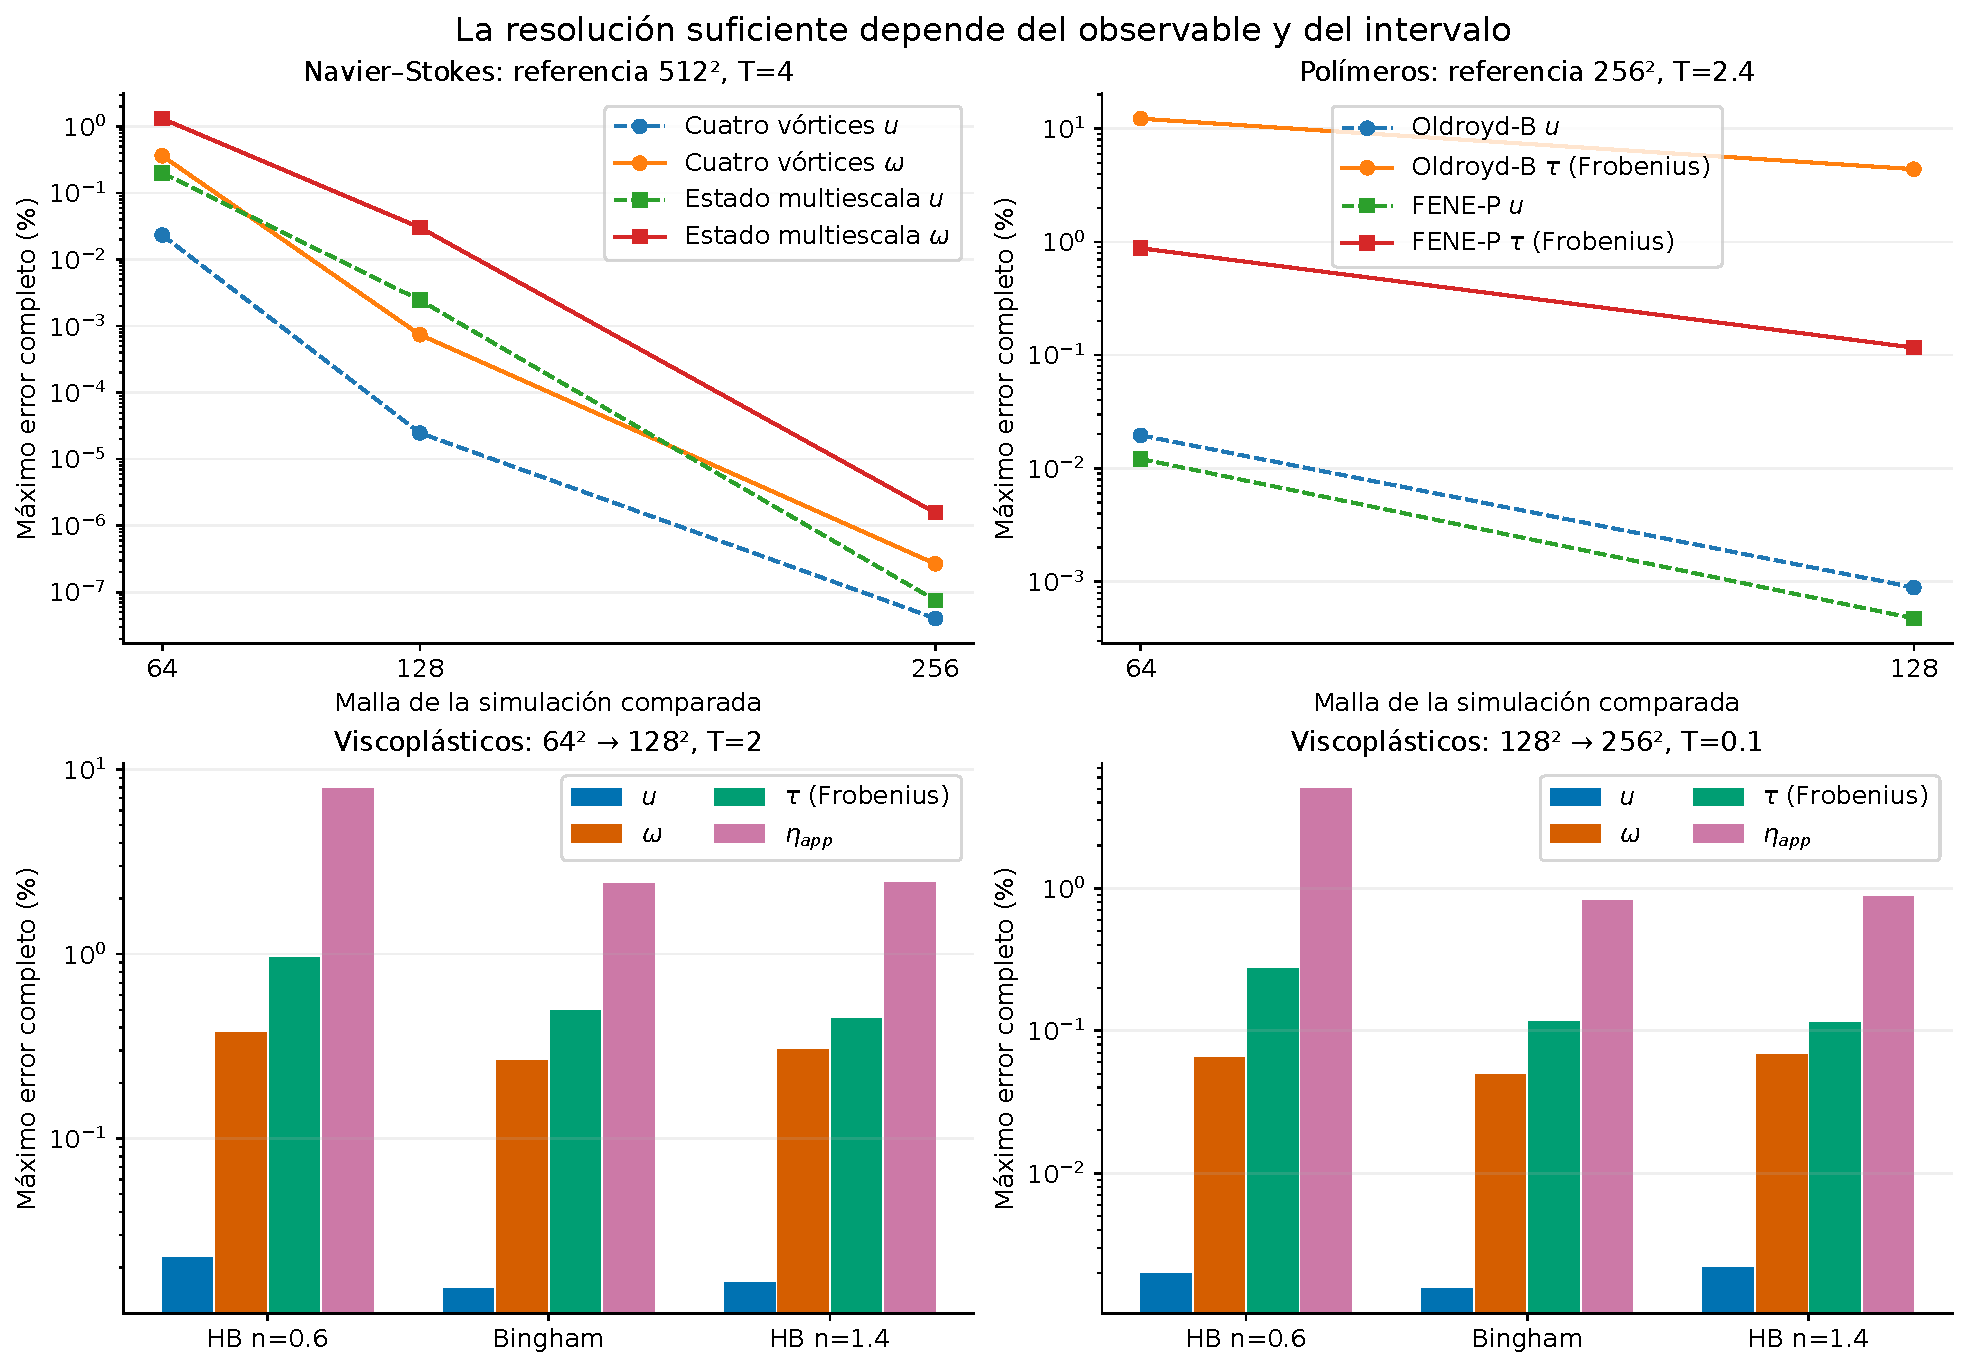
\includegraphics[width=\textwidth,height=.71\textheight,keepaspectratio]{results/research/reference_fidelity_2026-10-14/figures/fidelity_observable_grid.pdf}
\caption{Fidelidad por observable y malla. Cada serie compara integraciones independientes con su referencia fina, sobre el horizonte indicado. La velocidad y sus derivadas o cierres constitutivos requieren precisiones diferentes; una diferencia pequeña entre mallas del mismo solver no elimina posibles sesgos comunes.}
\label{fig:reference-credibility}\end{figure}
\clearpage

\subsection{Cómo modifica la referencia el error atribuido al estimador}

\begingroup\small\setlength{\tabcolsep}{3pt}
\begin{longtable}{@{}>{\raggedright\arraybackslash}p{4.5cm}>{\raggedright\arraybackslash}p{2.3cm}>{\raggedright\arraybackslash}p{2.0cm}>{\raggedright\arraybackslash}p{3.2cm}>{\raggedright\arraybackslash}p{2.3cm}@{}}
\caption{Presupuesto de error de vorticidad: la cota utiliza denominador y espacio fino comunes, mientras que el error frente a la solución gruesa conserva su normalización original.}\\
\toprule
\textbf{Ruido / método} & \textbf{Error vs. gruesa} & \textbf{Error ref.} & \textbf{Intervalo vs. fina} & \textbf{Medido vs. fina} \\
\midrule\endfirsthead
\toprule
\textbf{Ruido / método} & \textbf{Error vs. gruesa} & \textbf{Error ref.} & \textbf{Intervalo vs. fina} & \textbf{Medido vs. fina} \\
\midrule\endhead
gaussian\_iid / tls\_r8\_projected & 97.28~\% & 3.189e-04~\% & 97.28~\%–97.28~\% & 97.28~\% \\
gaussian\_iid / tls\_r8\_fixed\_band & 8.189~\% & 3.189e-04~\% & 8.188~\%–8.189~\% & 8.189~\% \\
gaussian\_iid / identity\_fixed\_band & 10.03~\% & 3.189e-04~\% & 10.03~\%–10.03~\% & 10.03~\% \\
spatial\_fixed\_length / tls\_r8\_projected & 39.67~\% & 3.189e-04~\% & 39.67~\%–39.67~\% & 39.67~\% \\
spatial\_fixed\_length / tls\_r8\_fixed\_band & 22.28~\% & 3.189e-04~\% & 22.28~\%–22.28~\% & 22.28~\% \\
spatial\_fixed\_length / identity\_fixed\_band & 48.77~\% & 3.189e-04~\% & 48.77~\%–48.77~\% & 48.77~\% \\
gaussian\_iid / tls\_r8\_projected & 199.6~\% & 1.557e-07~\% & 199.6~\%–199.6~\% & 199.6~\% \\
gaussian\_iid / tls\_r8\_fixed\_band & 7.108~\% & 1.557e-07~\% & 7.108~\%–7.108~\% & 7.108~\% \\
\bottomrule\end{longtable}\endgroup

\clearpage
\begin{figure}[p]\centering
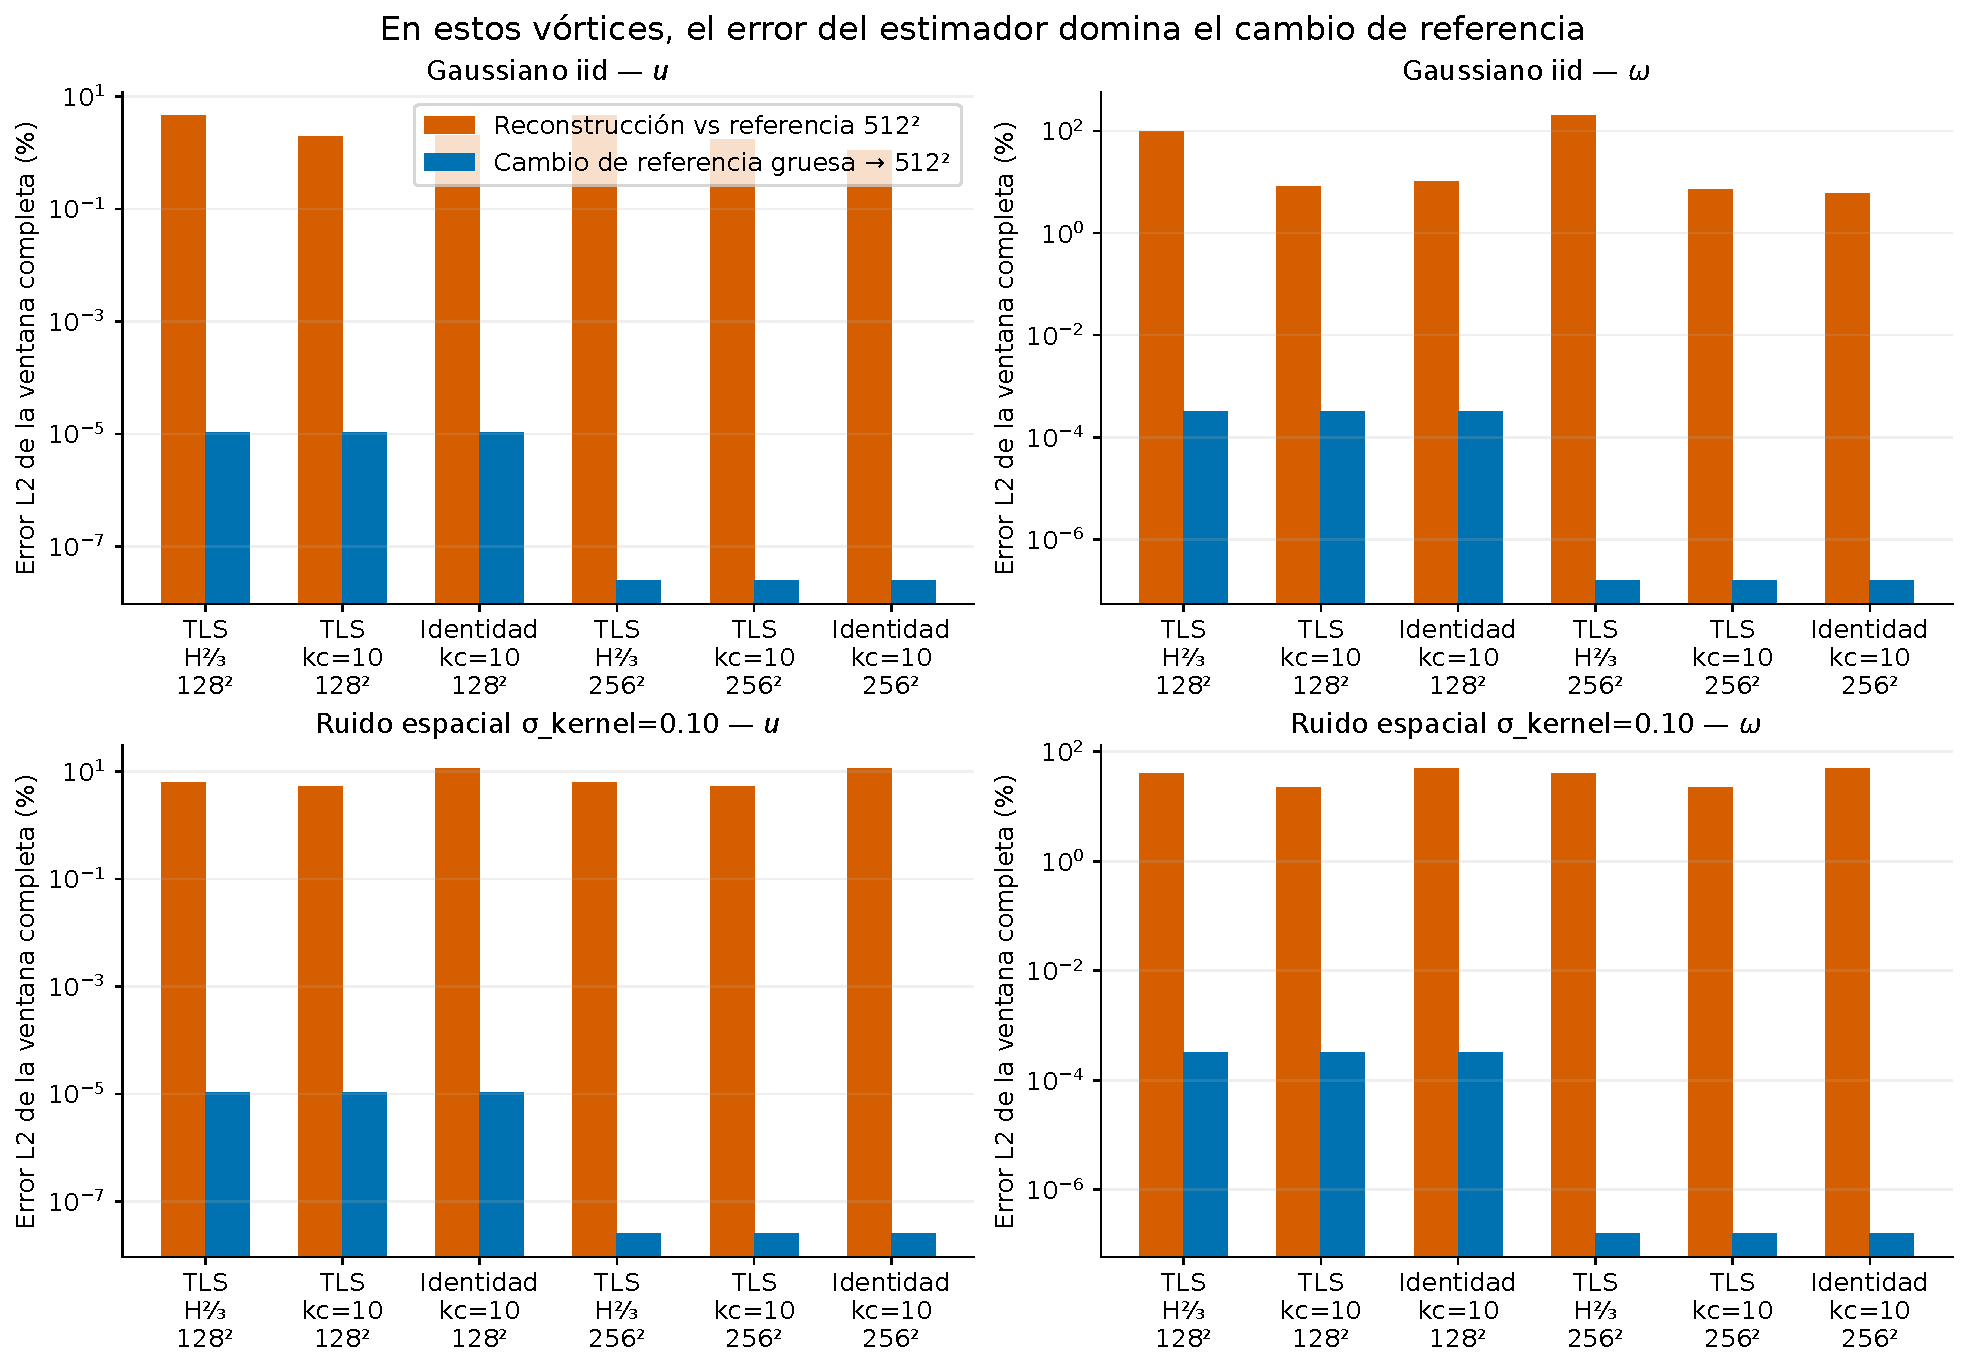
\includegraphics[width=\textwidth,height=.71\textheight,keepaspectratio]{results/research/reference_fidelity_2026-10-14/figures/reconstruction_error_budget.pdf}
\caption{Reconstrucción y discretización son fuentes de error distintas. Las cotas triangulares prolongan los campos al mismo espacio y normalizan por la referencia fina; no suman porcentajes con denominadores distintos. La referencia fina sigue siendo numérica y el intervalo describe discrepancia entre soluciones, no incertidumbre experimental.}
\label{fig:reconstruction-budget}\end{figure}
\clearpage

\clearpage
\begin{figure}[p]\centering
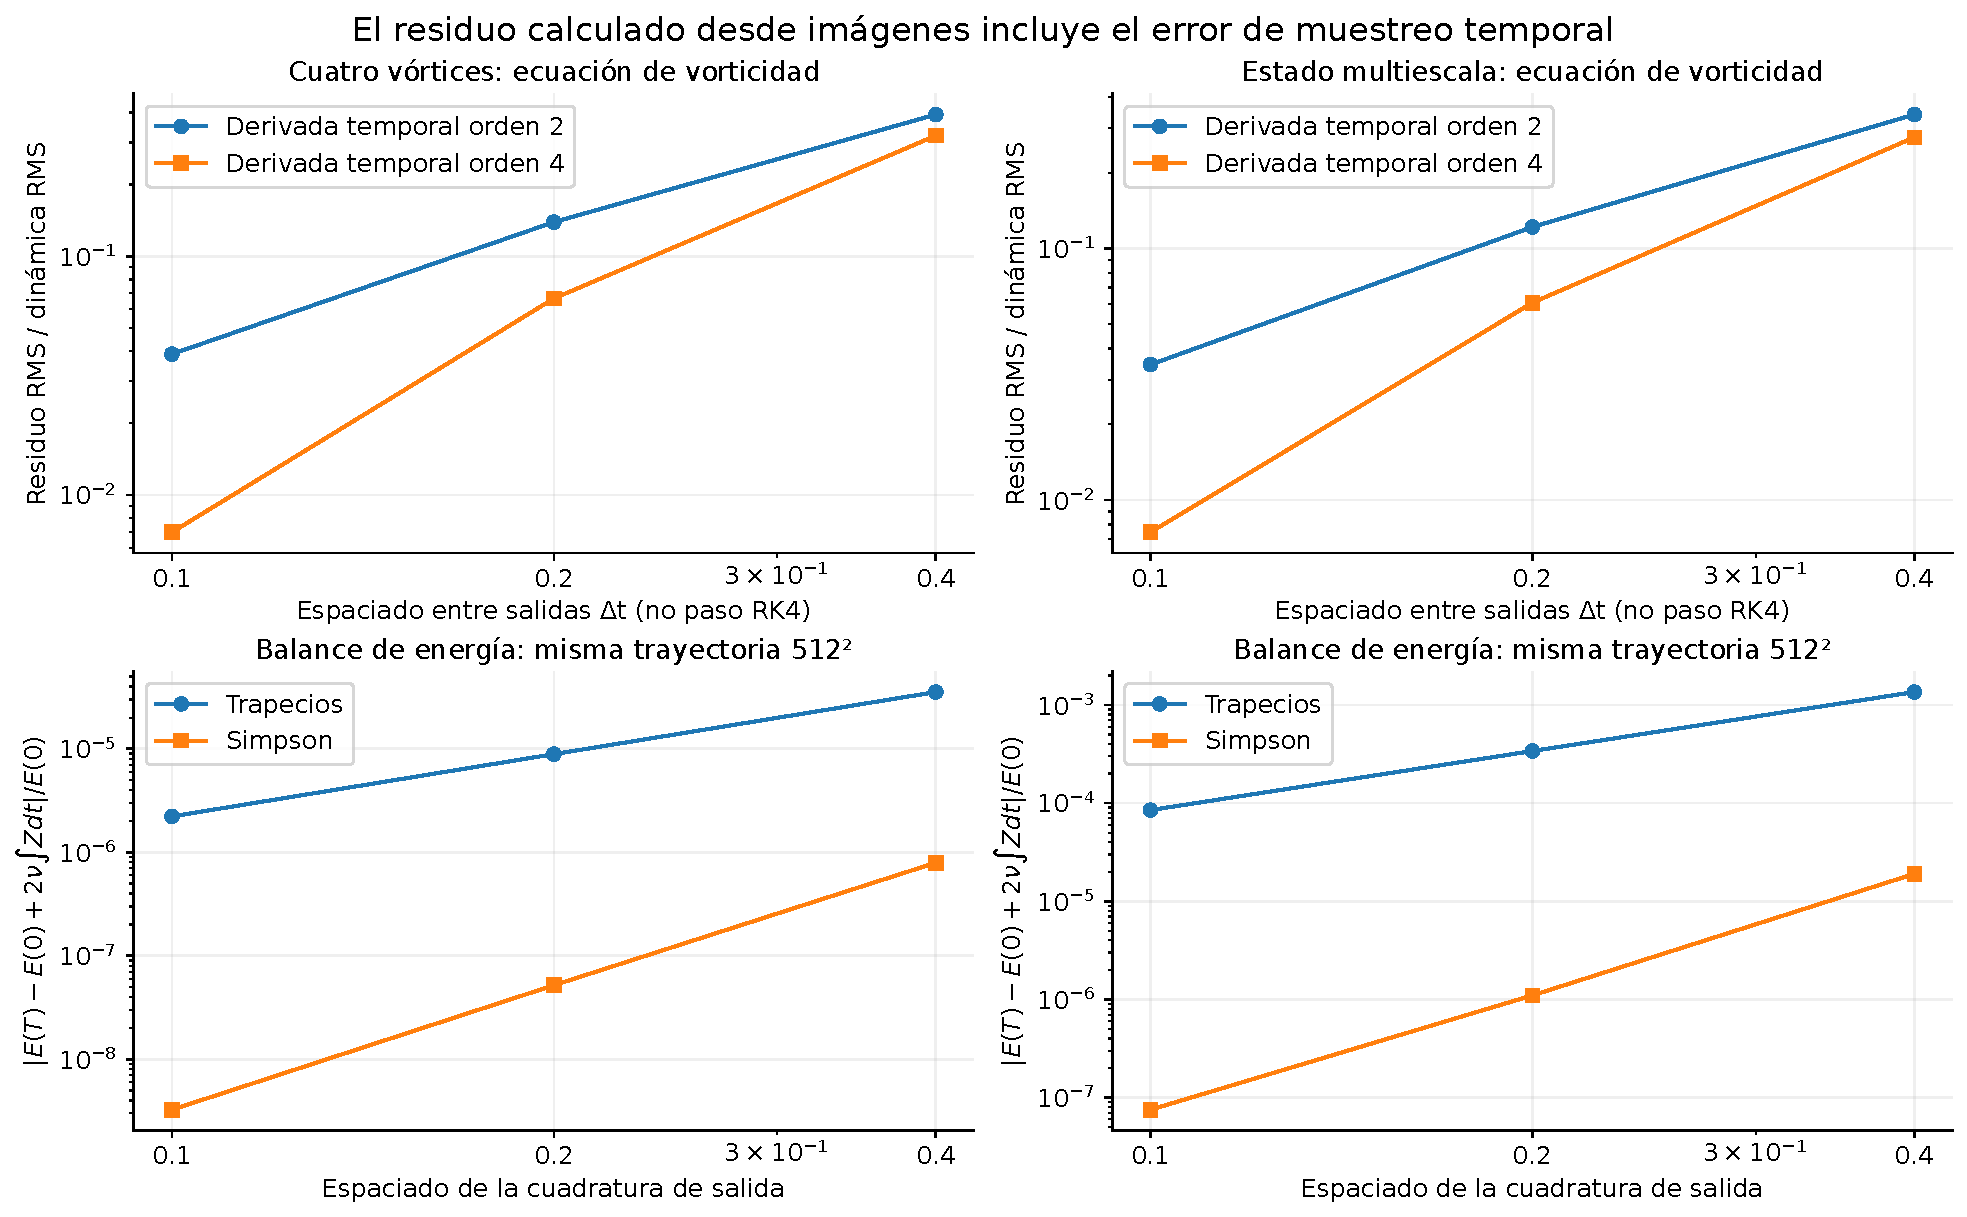
\includegraphics[width=\textwidth,height=.71\textheight,keepaspectratio]{results/research/reference_fidelity_2026-10-14/figures/residual_sampling.pdf}
\caption{Dependencia de los residuos con la separación entre estados guardados y el operador temporal. La misma trayectoria puede producir residuos distintos al muestrearse con menor frecuencia. Estos diagnósticos no equivalen al residuo de las etapas internas del integrador ni certifican el solver.}
\label{fig:sampled-residual}\end{figure}
\clearpage

\begingroup\small\setlength{\tabcolsep}{3pt}
\begin{longtable}{@{}>{\raggedright\arraybackslash}p{3.2cm}>{\raggedright\arraybackslash}p{2.9cm}>{\raggedright\arraybackslash}p{2.9cm}>{\raggedright\arraybackslash}p{2.7cm}>{\raggedright\arraybackslash}p{2.7cm}@{}}
\caption{Efecto del tratamiento de las mismas salidas cada 0.1: el residuo se normaliza por RMS de convección menos difusión sobre siete centros comunes entre t=0.8 y t=3.2; la energía usa el estado final t=4.}\\
\toprule
\textbf{Referencia 512$^2$} & \textbf{Residuo orden 2} & \textbf{Residuo orden 4} & \textbf{Trap. |$\Delta$E|/$E_0$} & \textbf{Simpson |$\Delta$E|/$E_0$} \\
\midrule\endfirsthead
\toprule
\textbf{Referencia 512$^2$} & \textbf{Residuo orden 2} & \textbf{Residuo orden 4} & \textbf{Trap. |$\Delta$E|/$E_0$} & \textbf{Simpson |$\Delta$E|/$E_0$} \\
\midrule\endhead
Vórtices NS & 3.892~\% & 0.6973~\% & 2.221e-06 & 3.251e-09 \\
Multiescala NS & 3.454~\% & 0.745~\% & 8.488e-05 & 7.517e-08 \\
\bottomrule\end{longtable}\endgroup

Esta normalización del residuo es la dinámica RMS de la propia trayectoria, distinta de la escala heurística de vorticidad utilizada en las métricas históricas. No se comparan directamente sus porcentajes. Cambiar stencil o cuadratura de salida puede reducir mucho el diagnóstico manteniendo exactamente la misma integración RK4: por tanto, el error de muestreo de salida debe separarse del error del solver.

\subsection{Aislar el muestreo dentro de una misma integración}

\begingroup\small\setlength{\tabcolsep}{3pt}
\begin{longtable}{@{}>{\raggedright\arraybackslash}p{3.3cm}>{\raggedright\arraybackslash}p{2.1cm}>{\raggedright\arraybackslash}p{2.6cm}>{\raggedright\arraybackslash}p{3.0cm}>{\raggedright\arraybackslash}p{3.4cm}@{}}
\caption{Una única integración nueva por caso guarda 161 estados cada 0.025; las demás cadencias son submuestras exactas. Orden temporal cuatro y normalización dinámica RMS comunes. La malla permanece en 128$^2$.}\\
\toprule
\textbf{Referencia 128$^2$} & \textbf{Separación de salida} & \textbf{Residuo completo} & \textbf{Componente temporal} & \textbf{Defecto de proyección} \\
\midrule\endfirsthead
\toprule
\textbf{Referencia 128$^2$} & \textbf{Separación de salida} & \textbf{Residuo completo} & \textbf{Componente temporal} & \textbf{Defecto de proyección} \\
\midrule\endhead
Vórtices NS & 0.1 & 0.6974~\% & 0.6973~\% & 0.01064~\% \\
Vórtices NS & 0.025 & 0.01116~\% & 0.003374~\% & 0.01064~\% \\
Multiescala NS & 0.1 & 0.85~\% & 0.7449~\% & 0.4093~\% \\
Multiescala NS & 0.025 & 0.4093~\% & 0.004041~\% & 0.4093~\% \\
\bottomrule\end{longtable}\endgroup

Al guardar más estados, la componente temporal del residuo disminuye mientras el defecto de proyección espacial conserva su valor. El residuo completo alcanza así un piso asociado al operador discreto de esa malla. Las 161 salidas y sus submuestras proceden de una misma integración, por lo que no son nuevas realizaciones físicas. El contraste contra la integración original a tiempos comunes verifica por separado el pequeño cambio de paso interno. Esta prueba 128$^2$ se mantiene distinta de los residuos 512$^2$ anteriores.

\clearpage
\begin{landscape}
\begin{figure}[p]\centering
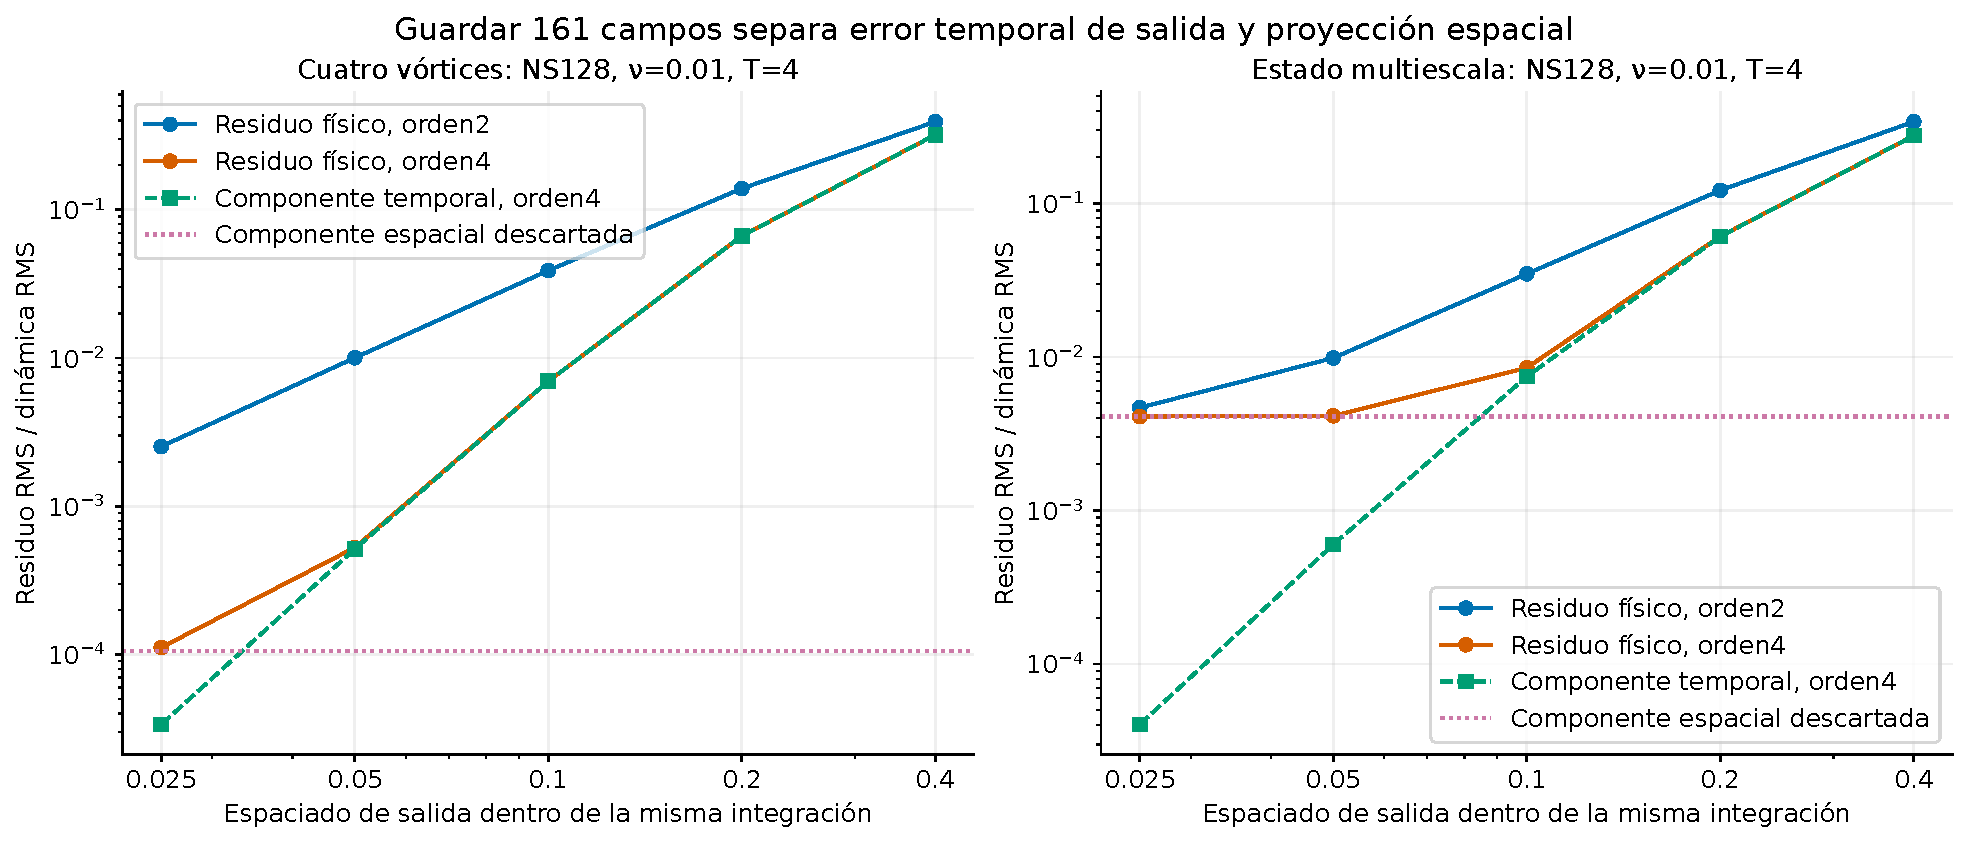
\includegraphics[width=\linewidth,height=.80\textwidth,keepaspectratio]{results/research/reference_fidelity_2026-10-14/figures/dense_sampling_isolation.pdf}
\caption{Aislamiento del muestreo temporal sobre dos integraciones 128$^2$ con 161 estados. Al reducir la separación entre salidas disminuye el error de diferenciación, mientras la proyección espacial fija un piso de residuo. La normalización y los centros temporales son comunes dentro de cada caso; el gráfico no atribuye a RK4 un defecto producido por guardar pocas instantáneas.}
\label{fig:dense-output-isolation}\end{figure}
\end{landscape}
\clearpage

\clearpage
\section{Comparación pareada de modelos sobre la misma observación}

El banco principal registra 1050 ajustes y 3150 evaluaciones: 105 observaciones compartidas por diez estimadores y tres salidas físicas. Se utilizan siete referencias 128$^2$, cinco ruidos al 20~\% RMS y semillas nuevas 101, 307 y 911. Los estimadores reciben sólo observación, tiempo, geometría y parámetros declarados; el limpio evalúa después. Raw, H y H+B comparten cada ajuste, por lo que sus evaluaciones no añaden entrenamientos ni nuevas realizaciones de ruido.

\begingroup\small\setlength{\tabcolsep}{3pt}
\begin{longtable}{@{}>{\raggedright\arraybackslash}p{3.9822cm}>{\raggedright\arraybackslash}p{1.5929cm}>{\raggedright\arraybackslash}p{1.792cm}>{\raggedright\arraybackslash}p{1.6427cm}>{\raggedright\arraybackslash}p{1.8916cm}>{\raggedright\arraybackslash}p{1.7422cm}>{\raggedright\arraybackslash}p{1.9911cm}@{}}
\caption{Panel de configuraciones fijas: medianas de salidas finitas, incluidas las no convergentes identificadas, y conteos de aceptación conjunta. La distribución mezcla casos y ruidos; no constituye una clasificación universal ni sustituye las tablas estratificadas.}\\
\toprule
\textbf{Estimador} & \textbf{Raw $e_u$} & \textbf{Raw $e_\omega$} & \textbf{Raw adm.} & \textbf{H+B $e_\omega$} & \textbf{H+B adm.} & \textbf{Fallo / no conv.} \\
\midrule\endfirsthead
\toprule
\textbf{Estimador} & \textbf{Raw $e_u$} & \textbf{Raw $e_\omega$} & \textbf{Raw adm.} & \textbf{H+B $e_\omega$} & \textbf{H+B adm.} & \textbf{Fallo / no conv.} \\
\midrule\endhead
Identity & 20~\% & 498.1~\% & 0/105 & 9.963~\% & 87/105 & 0 \\
POD r=8 & 12.84~\% & 309.7~\% & 0/105 & 9.231~\% & 90/105 & 0 \\
DMD r=8 & 9.729~\% & 230~\% & 0/105 & 9.251~\% & 105/105 & 0 \\
TLS-DMD r=8 & 10.29~\% & 247~\% & 0/105 & 9.994~\% & 93/105 & 0 \\
RPCA/PCP & 12.96~\% & 62.85~\% & 3/105 & 16.54~\% & 80/105 & 0 \\
RPCA estable & 10~\% & 143.1~\% & 0/105 & 15.44~\% & 105/105 & 0 \\
Outlier Pursuit & 39.04~\% & 87.6~\% & 0/105 & 50.22~\% & 0/105 & 0 \\
PCP + TLS-DMD & 13.04~\% & 63.05~\% & 3/105 & 17.37~\% & 77/105 & 0 \\
RPCA estable + TLS-DMD & 10.06~\% & 142.1~\% & 0/105 & 15.17~\% & 102/105 & 0 \\
Optimized DMD r=8 & 10.7~\% & 251.2~\% & 0/105 & 9.014~\% & 86/105 & 8 \\
\bottomrule\end{longtable}\endgroup

Se conservan 0 ajustes fallidos y 8 ajustes no convergentes. Los fallos no se reemplazan por el mejor inicio ni se borran de los denominadores. El rango ocho es un presupuesto de los métodos modales; PCP, RPCA estable y Outlier Pursuit producen rangos efectivos por sus regularizadores. Una norma observada menor no demuestra que el modelo haya identificado mejor la señal limpia.

\clearpage
\begin{landscape}
\begin{figure}[p]\centering
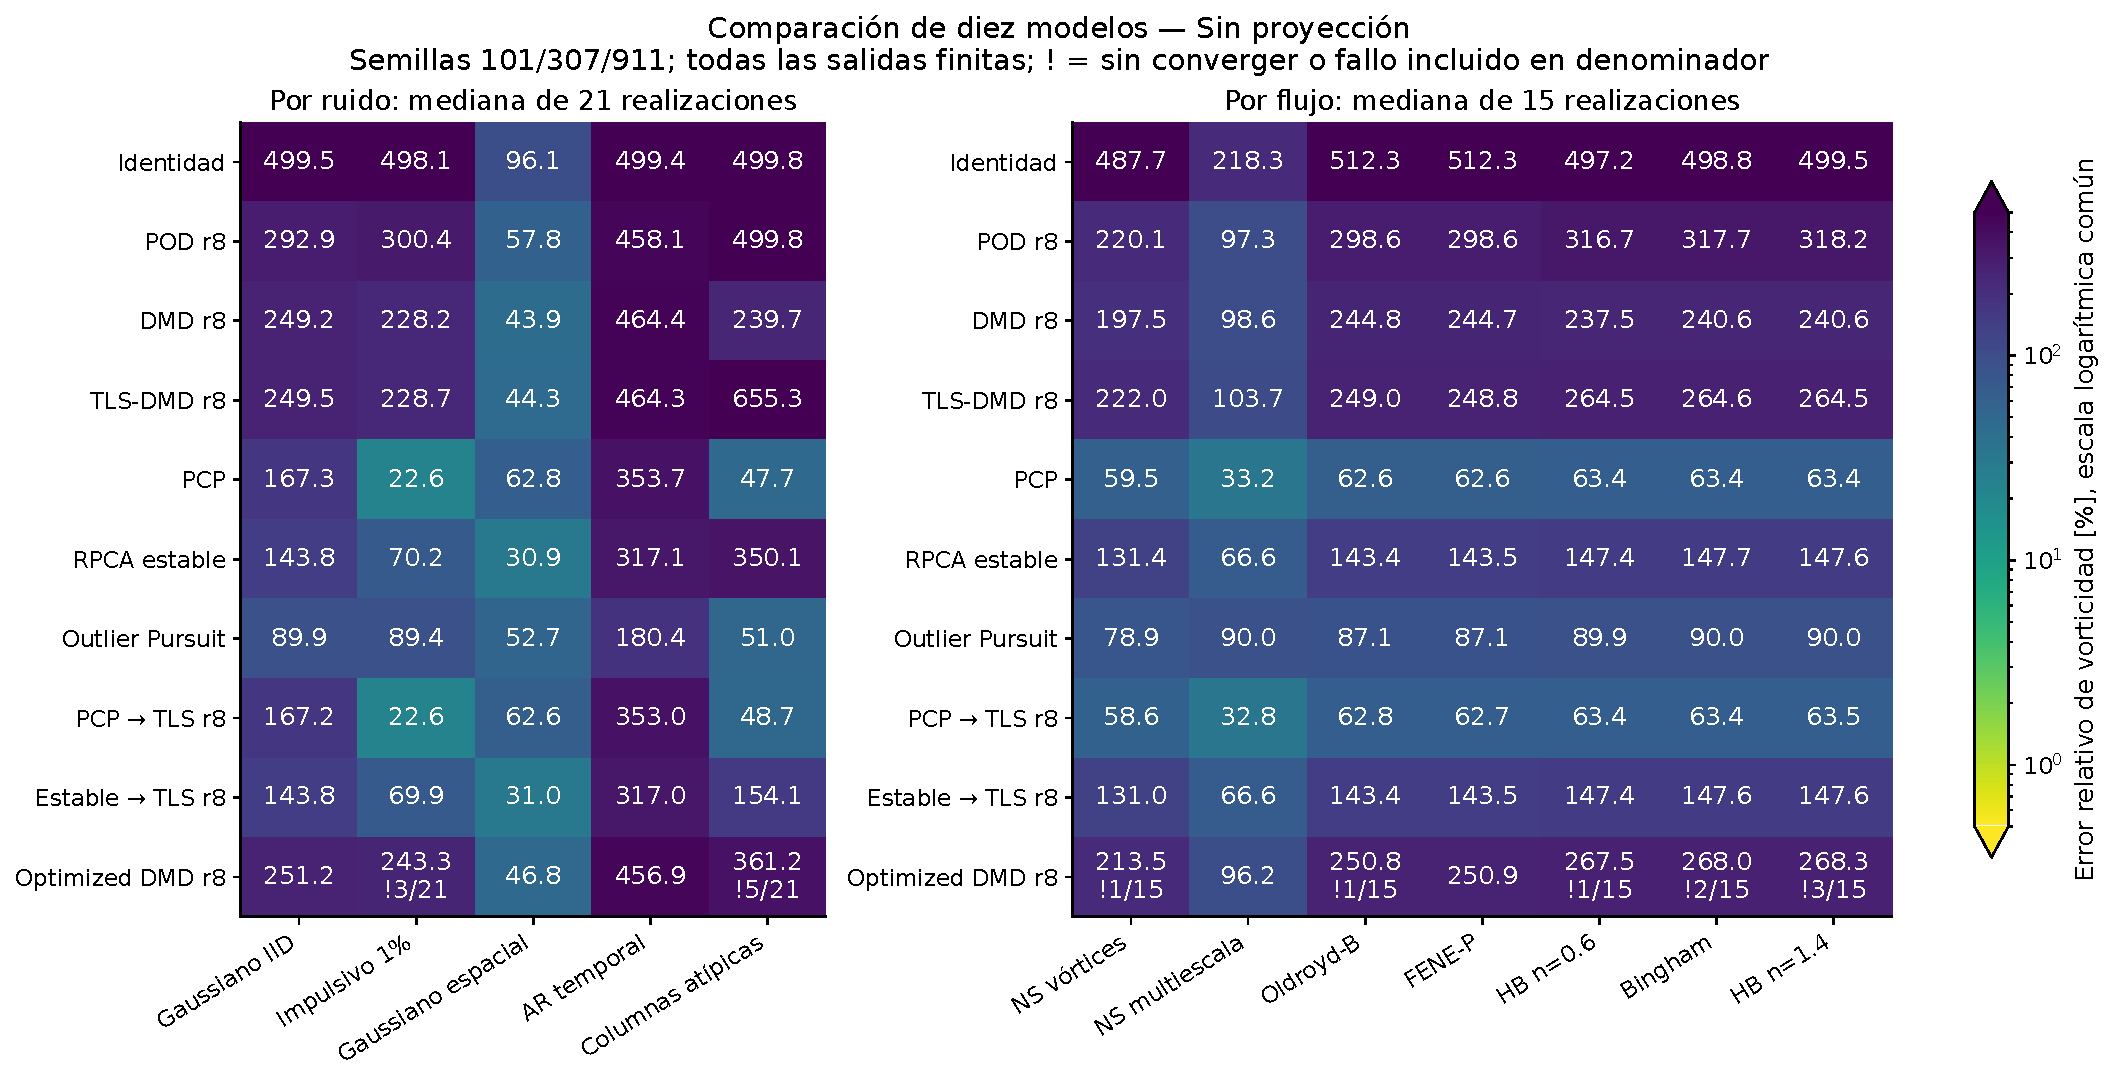
\includegraphics[width=\linewidth,height=.80\textwidth,keepaspectratio]{results/research/model_fidelity_benchmark_2026-10-14/figures/model_raw_overview.pdf}
\caption{Comparación sin posprocesamiento físico. Los errores de vorticidad se calculan con el mismo operador para cada referencia y estimación. La estratificación revela ventajas condicionadas a contaminación y dinámica; los marcadores de fallo y no convergencia permanecen diferenciados de un error grande.}
\label{fig:models-raw}\end{figure}
\end{landscape}
\clearpage

\subsection{Qué controla cada familia de estimadores}

POD controla compresión espacial-temporal, sin imponer una evolución autónoma. DMD y TLS-DMD ajustan una dinámica lineal reducida; TLS trata ruido en ambos bloques consecutivos. PCP separa bajo rango y entradas dispersas; Outlier Pursuit separa columnas corruptas completas. RPCA estable admite un residuo denso, con regularización heurística informada por la intensidad sintética conocida. Las cadenas PCP/TLS y RPCA estable/TLS permiten preguntar si la limpieza previa ayuda o si introduce sesgo que el ajuste dinámico amplifica. Estas funciones diferentes justifican comparar errores y recursos, sin transformar sus hipótesis en promesas de superioridad.

La corrupción de columnas necesita un criterio específico: recuperar el subespacio no identifica por sí solo cada valor limpio oculto en un estado totalmente corrupto. Los errores en esas instantáneas siguen incluidos. Una trayectoria de velocidad más regular puede favorecer bajo rango sin representar mejor memoria de esfuerzo, viscosidad o dinámica física; por ello se examinan observables derivados por separado.

\subsection{Control sin ruido: sesgo del modelo y de su regularización}

El control sin contaminación realiza 84 ajustes deterministas y 252 evaluaciones sobre las mismas siete trayectorias, con 0 fallos y 0 ajustes no convergentes. Setenta ajustes heredan las configuraciones del banco principal. En RPCA estable, aplicar el presupuesto de ruido del 20~\% a una observación sin ruido es una prueba deliberada de sesgo por regularización; no representa calibración correcta de ruido cero. Los catorce ajustes adicionales informan intensidad conocida cero para RPCA estable y su cadena TLS, sin cambiar rango, tolerancia ni límites.

\begingroup\small\setlength{\tabcolsep}{3pt}
\begin{longtable}{@{}>{\raggedright\arraybackslash}p{3.0cm}>{\raggedright\arraybackslash}p{2.2cm}>{\raggedright\arraybackslash}p{2.2cm}>{\raggedright\arraybackslash}p{2.2cm}>{\raggedright\arraybackslash}p{2.7cm}>{\raggedright\arraybackslash}p{2.3cm}@{}}
\caption{Sesgo Raw sin ruido de observación. Las dos columnas de RPCA estable separan el presupuesto heredado del control de ruido conocido cero. Se conservan salidas finitas; la figura identifica las no convergentes.}\\
\toprule
\textbf{Referencia} & \textbf{PCP $e_\omega$} & \textbf{OP $e_\omega$} & \textbf{TLS $e_\omega$} & \textbf{RPCA estable, 20~\%} & \textbf{RPCA estable, 0} \\
\midrule\endfirsthead
\toprule
\textbf{Referencia} & \textbf{PCP $e_\omega$} & \textbf{OP $e_\omega$} & \textbf{TLS $e_\omega$} & \textbf{RPCA estable, 20~\%} & \textbf{RPCA estable, 0} \\
\midrule\endhead
Vórtices NS & 17.38~\% & 61.57~\% & 5.543~\% & 18.35~\% & 2.329e-12~\% \\
Multiescala NS & 9.643~\% & 87.07~\% & 5.283~\% & 13.84~\% & 1.142e-12~\% \\
Oldroyd-B & 14.59~\% & 47.43~\% & 1.131~\% & 14.02~\% & 2.336e-12~\% \\
FENE-P & 14.67~\% & 47.46~\% & 0.9786~\% & 14.06~\% & 2.698e-12~\% \\
HB n=0.6 & 16.51~\% & 44.92~\% & 1.306~\% & 14.39~\% & 1.749e-12~\% \\
Bingham & 16.44~\% & 44.41~\% & 0.8647~\% & 14.36~\% & 1.924e-12~\% \\
HB n=1.4 & 16.5~\% & 44.05~\% & 0.6952~\% & 14.46~\% & 1.577e-12~\% \\
\bottomrule\end{longtable}\endgroup

Un error presente antes de añadir ruido no puede atribuirse a la contaminación. POD y DMD introducen restricciones de representación; PCP y Outlier Pursuit pueden asignar parte de la señal física a su componente de corrupción cuando sus supuestos no describen esa trayectoria. RPCA estable introduce además sesgo por umbralización. El control de presupuesto cero distingue esa regla de regularización de la dificultad dinámica: con penalizaciones cero el objetivo tiene múltiples minimizadores L+S=M. La implementación, iniciada con componente dispersa cero, devuelve aproximadamente identity; su cadena TLS mantiene la restricción modal. La fracción de entradas dispersas puede contar redondeo aunque su norma sea despreciable; no mide ruido inyectado en este control. Estos controles explican mecanismos sin escoger parámetros por menor error limpio.

\clearpage
\begin{landscape}
\begin{figure}[p]\centering
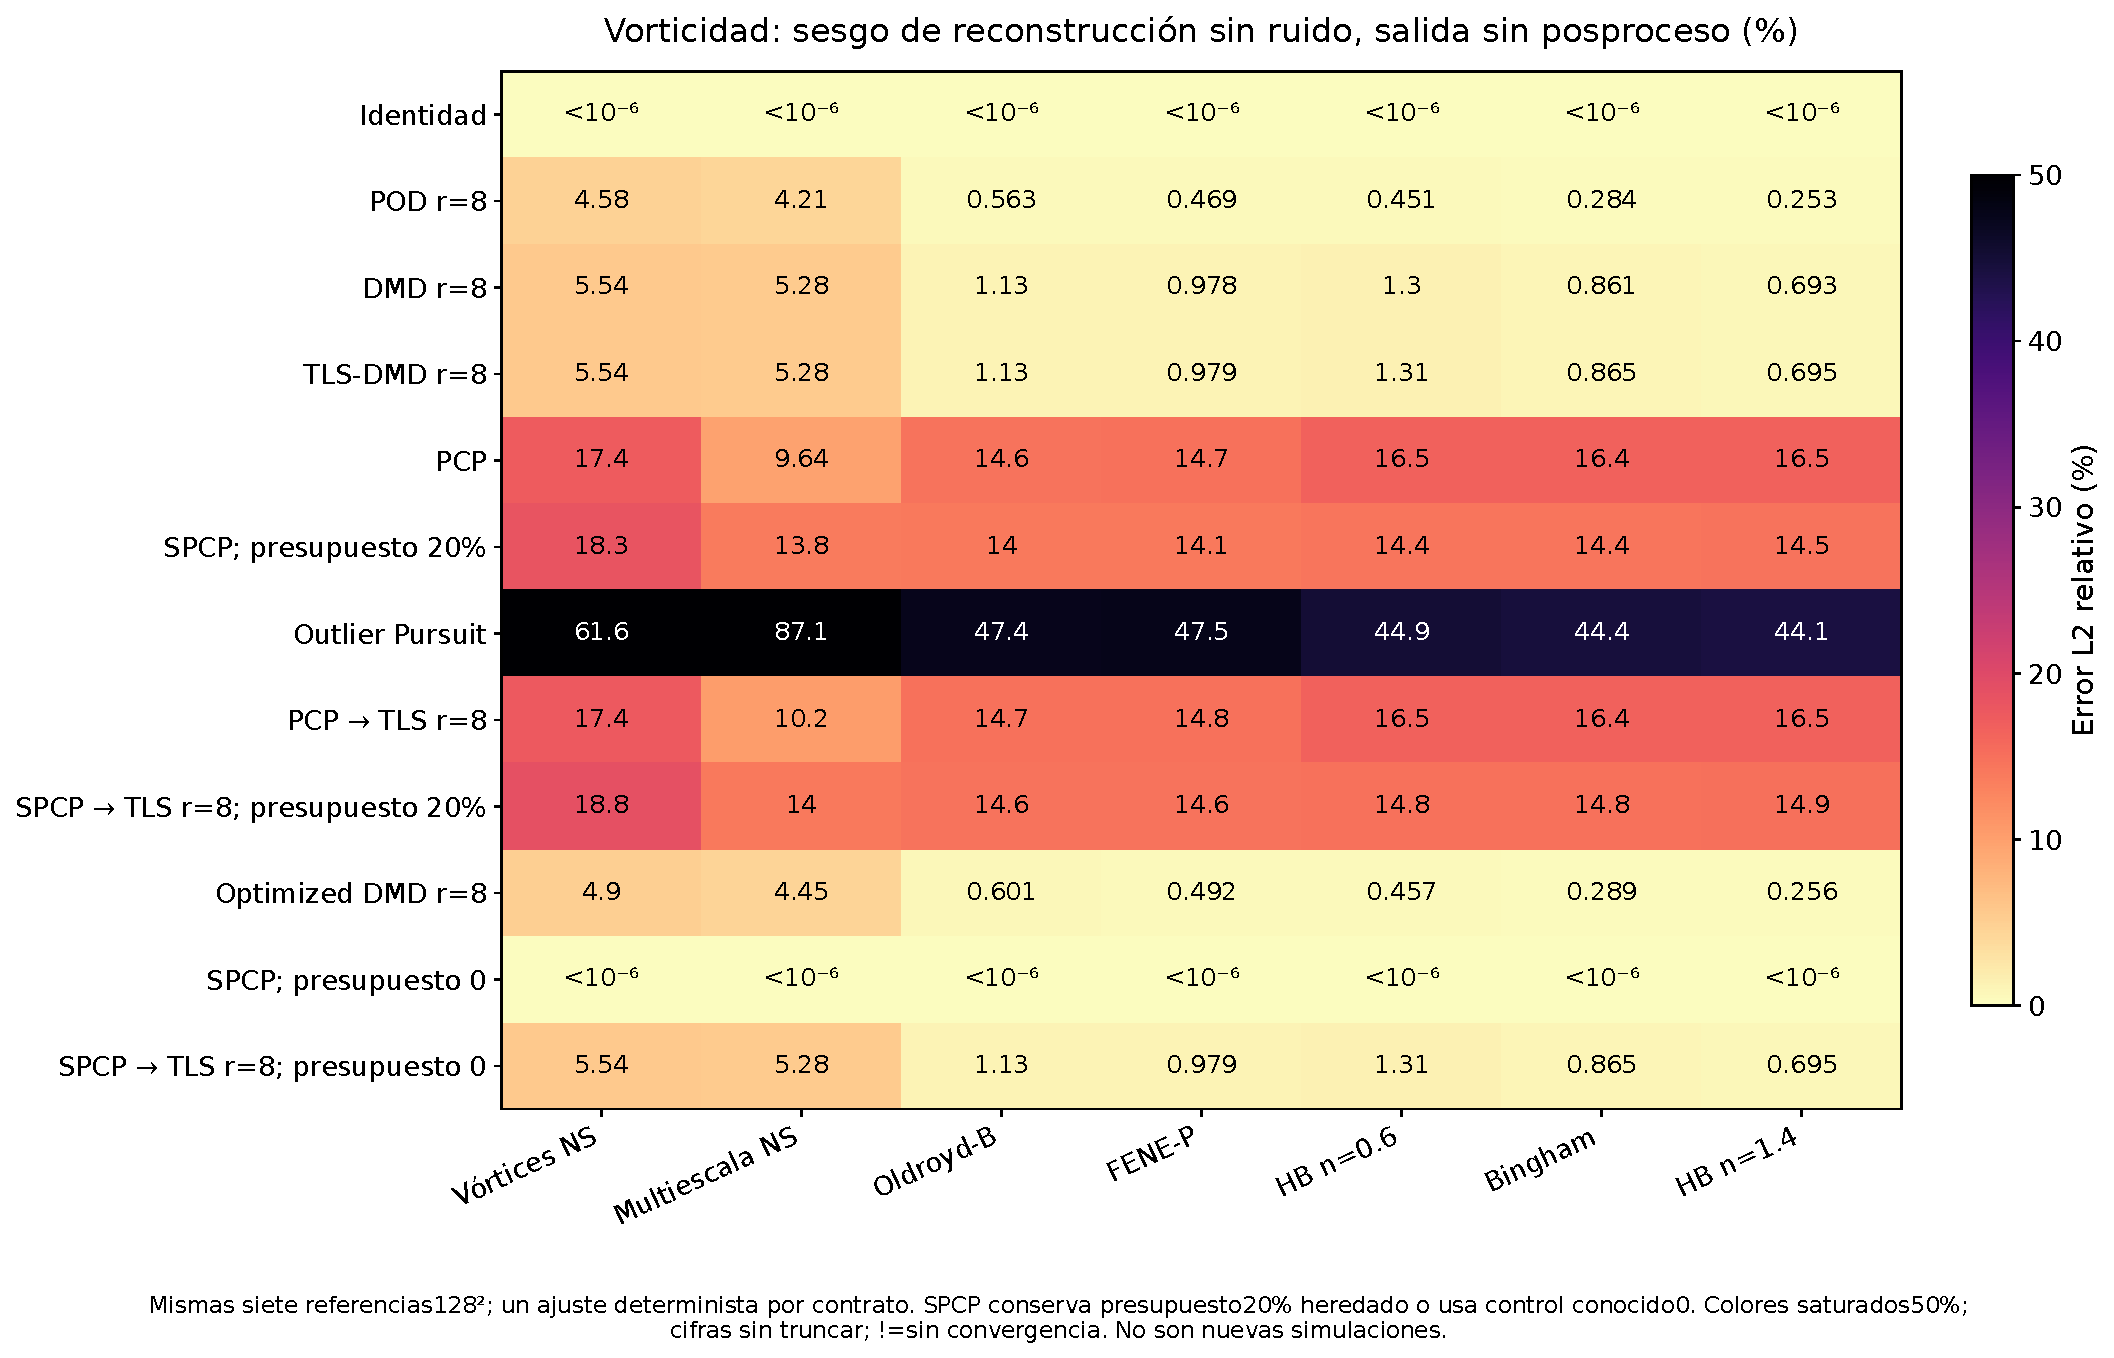
\includegraphics[width=\linewidth,height=.80\textwidth,keepaspectratio]{results/research/clean_model_controls_2026-10-14/figures/clean_bias_vorticity.pdf}
\caption{Error de vorticidad en observaciones sin ruido sobre las mismas siete referencias. Las configuraciones modales y las nucleares tienen presupuestos diferentes; el rango solicitado ocho no limita el rango de PCP u Outlier Pursuit. Los presupuestos 20~\% y cero de RPCA estable permanecen etiquetados, junto con convergencia.}
\label{fig:clean-model-bias}\end{figure}
\end{landscape}
\clearpage

\clearpage
\begin{landscape}
\begin{figure}[p]\centering
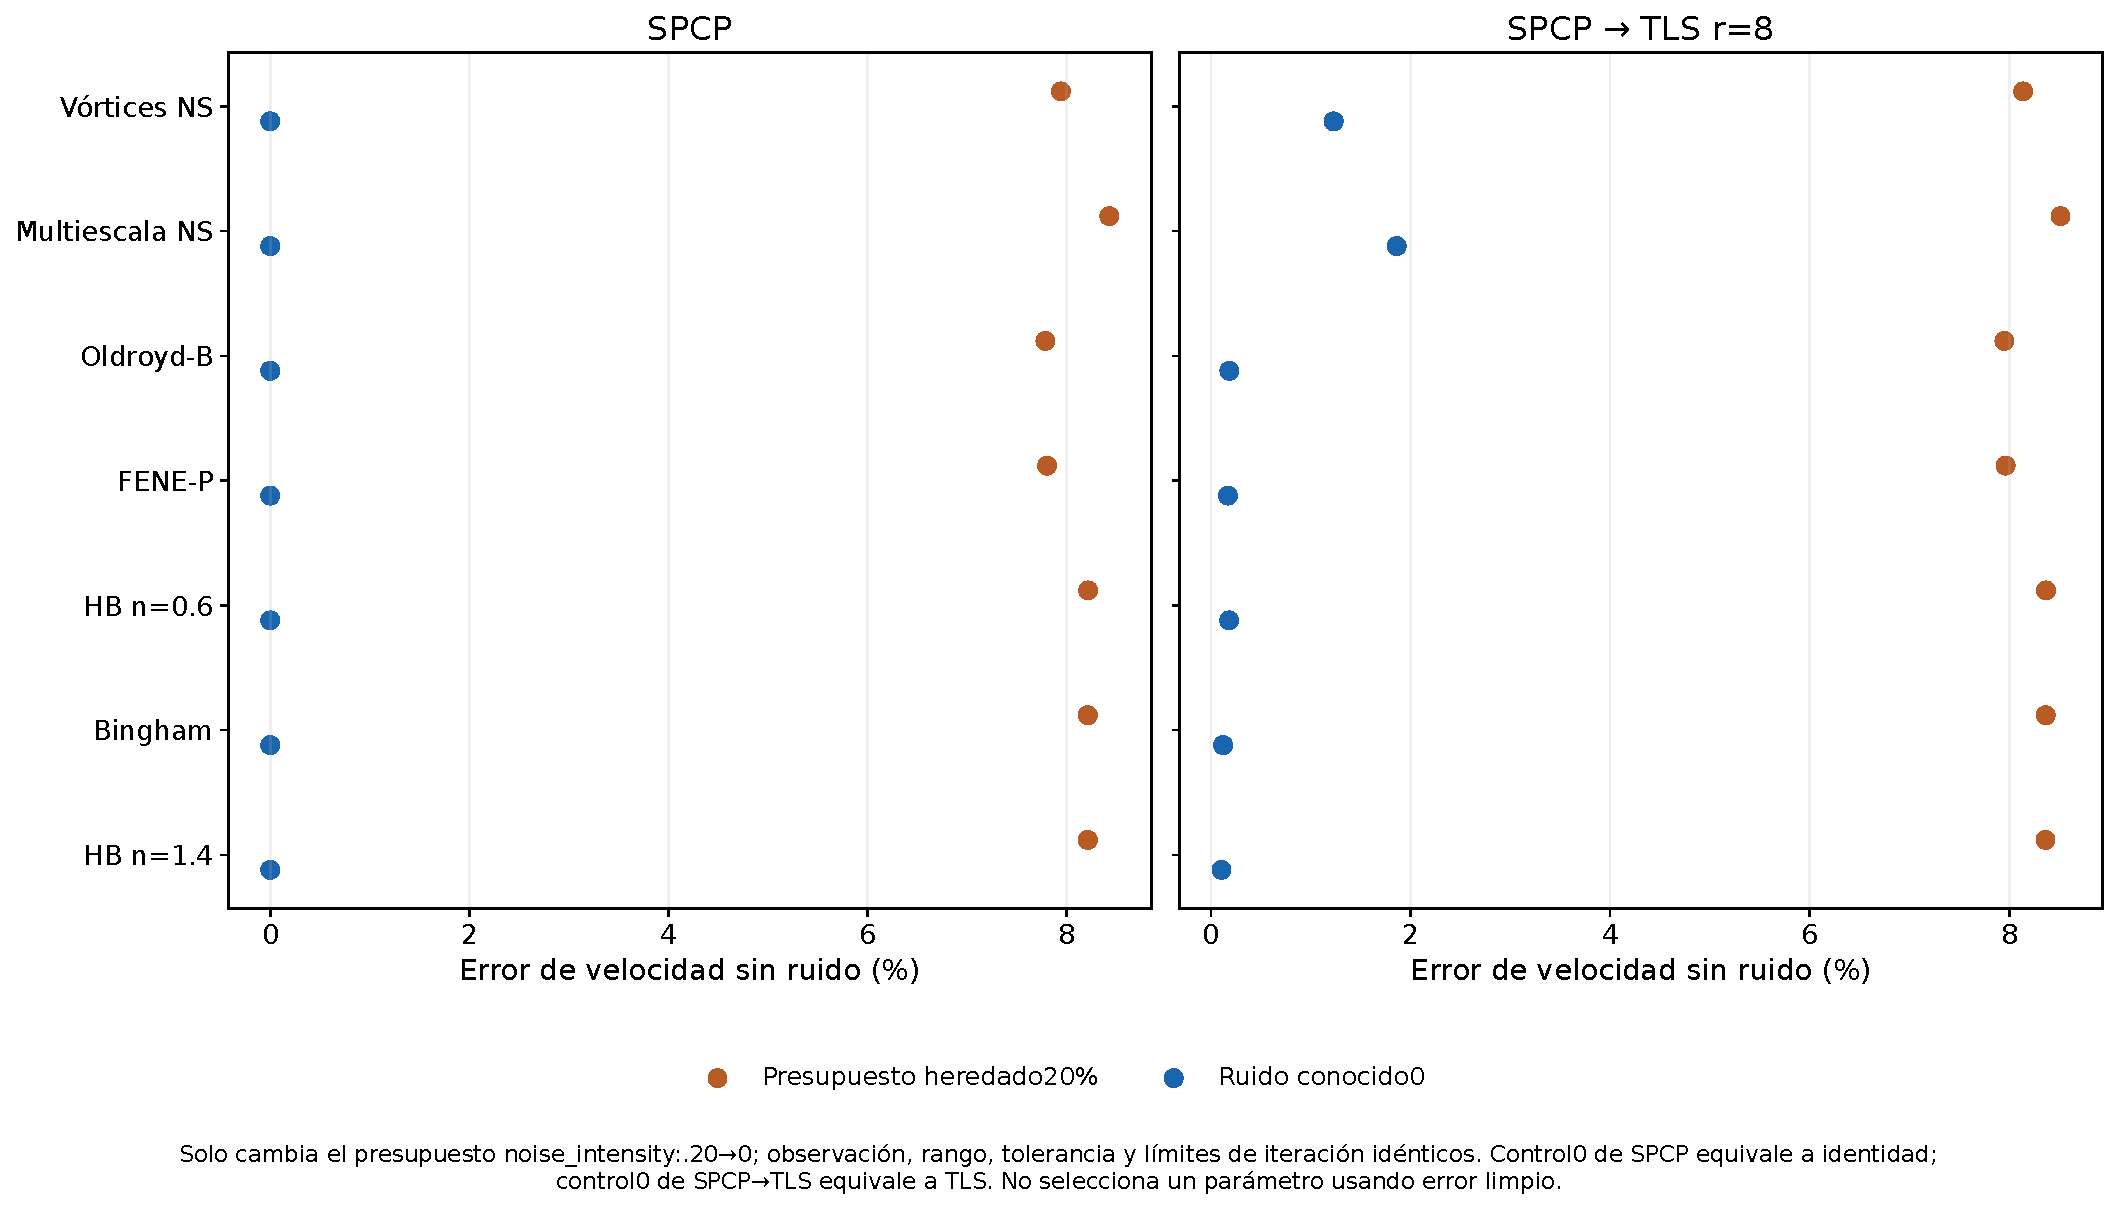
\includegraphics[width=\linewidth,height=.80\textwidth,keepaspectratio]{results/research/clean_model_controls_2026-10-14/figures/regularization_controls.pdf}
\caption{Control de la intensidad informada a la regularización: de 20~\% heredado a ruido conocido cero, con la misma observación limpia. El contraste identifica sesgo de la regla de umbralización y de la cadena modal; no modifica el protocolo del banco contaminado ni convierte el control en una calibración PIV real.}
\label{fig:regularization-contract}\end{figure}
\end{landscape}
\clearpage

\clearpage
\begin{landscape}
\begin{figure}[p]\centering
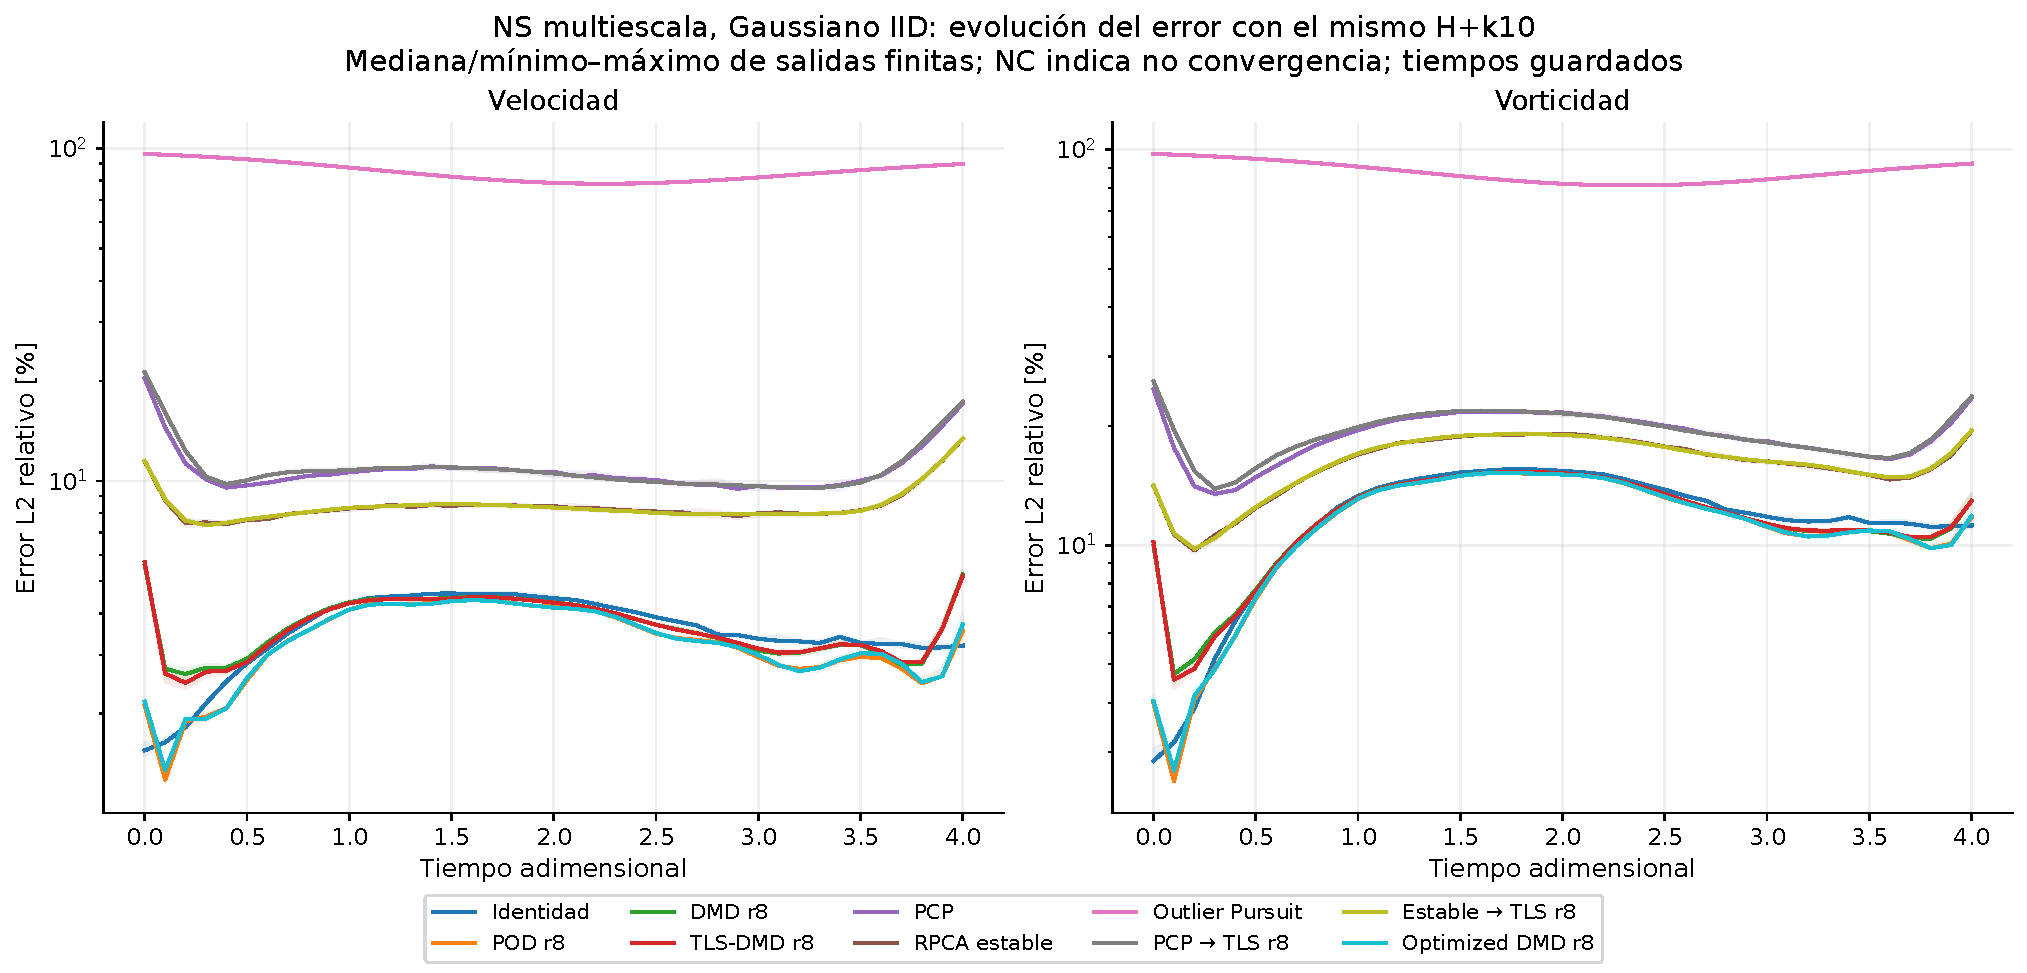
\includegraphics[width=\linewidth,height=.80\textwidth,keepaspectratio]{results/research/model_fidelity_benchmark_2026-10-14/figures/model_evolution_ns_multiscale_gaussian_iid.pdf}
\caption{Errores de reconstrucción durante la misma evolución multiescala newtoniana. Comparar estados intermedios permite detectar un deterioro que la norma global o el último estado pueden ocultar. Las curvas pertenecen al intervalo ajustado y no constituyen un pronóstico independiente.}
\label{fig:model-temporal-fidelity}\end{figure}
\end{landscape}
\clearpage

\clearpage
\section{Ablación física: qué añade el modelo sobre proyección y filtrado}

\begingroup\small\setlength{\tabcolsep}{3pt}
\begin{longtable}{@{}>{\raggedright\arraybackslash}p{4.0cm}>{\raggedright\arraybackslash}p{3.2cm}>{\raggedright\arraybackslash}p{2.4cm}>{\raggedright\arraybackslash}p{2.4cm}>{\raggedright\arraybackslash}p{2.4cm}@{}}
\caption{Ablación pareada de la misma estimación: diferencias en puntos porcentuales (pp), negativas cuando favorecen la operación añadida; el último conteo usa vorticidad y tolerancia de empate de $10^{-10}$, sin equivaler a aceptación conjunta.}\\
\toprule
\textbf{Estimador} & \textbf{Admisibles Raw$\to$H$\to$H+B} & \textbf{$\Delta$ $e_\omega$ por H} & \textbf{$\Delta$ $e_\omega$ por B} & \textbf{Supera identity H+B} \\
\midrule\endfirsthead
\toprule
\textbf{Estimador} & \textbf{Admisibles Raw$\to$H$\to$H+B} & \textbf{$\Delta$ $e_\omega$ por H} & \textbf{$\Delta$ $e_\omega$ por B} & \textbf{Supera identity H+B} \\
\midrule\endhead
Identity & 0 $\to$ 0 $\to$ 87 & 0 pp & -488.3 pp & 0/105 \\
POD r=8 & 0 $\to$ 3 $\to$ 90 & 0 pp & -303.2 pp & 81/105 \\
DMD r=8 & 0 $\to$ 3 $\to$ 105 & 0 pp & -223 pp & 85/105 \\
TLS-DMD r=8 & 0 $\to$ 3 $\to$ 93 & 0 pp & -239.2 pp & 72/105 \\
RPCA/PCP & 3 $\to$ 13 $\to$ 80 & 0 pp & -38.16 pp & 21/105 \\
RPCA estable & 0 $\to$ 3 $\to$ 105 & 0 pp & -129.8 pp & 21/105 \\
Outlier Pursuit & 0 $\to$ 0 $\to$ 0 & 0 pp & -14.11 pp & 13/105 \\
PCP + TLS-DMD & 3 $\to$ 13 $\to$ 77 & 0 pp & -37.62 pp & 19/105 \\
RPCA estable + TLS-DMD & 0 $\to$ 3 $\to$ 102 & 0 pp & -126.8 pp & 21/105 \\
Optimized DMD r=8 & 0 $\to$ 3 $\to$ 86 & 0 pp & -245.8 pp & 92/105 \\
\bottomrule\end{longtable}\endgroup

Helmholtz impone solenoidalidad y puede aumentar la admisibilidad aun cuando la vorticidad no cambia. Esa mejora informa el cumplimiento de una restricción, no una recuperación adicional de estructuras vorticales. El filtro de banda elimina gradientes de ruido y puede aumentar mucho más la fidelidad de vorticidad. Su control identity H+B establece cuánto se logra sin estimar ninguna dinámica. Las diferencias pareadas anteriores no se sustituyen por restar medianas independientes.

\clearpage
\begin{landscape}
\begin{figure}[p]\centering
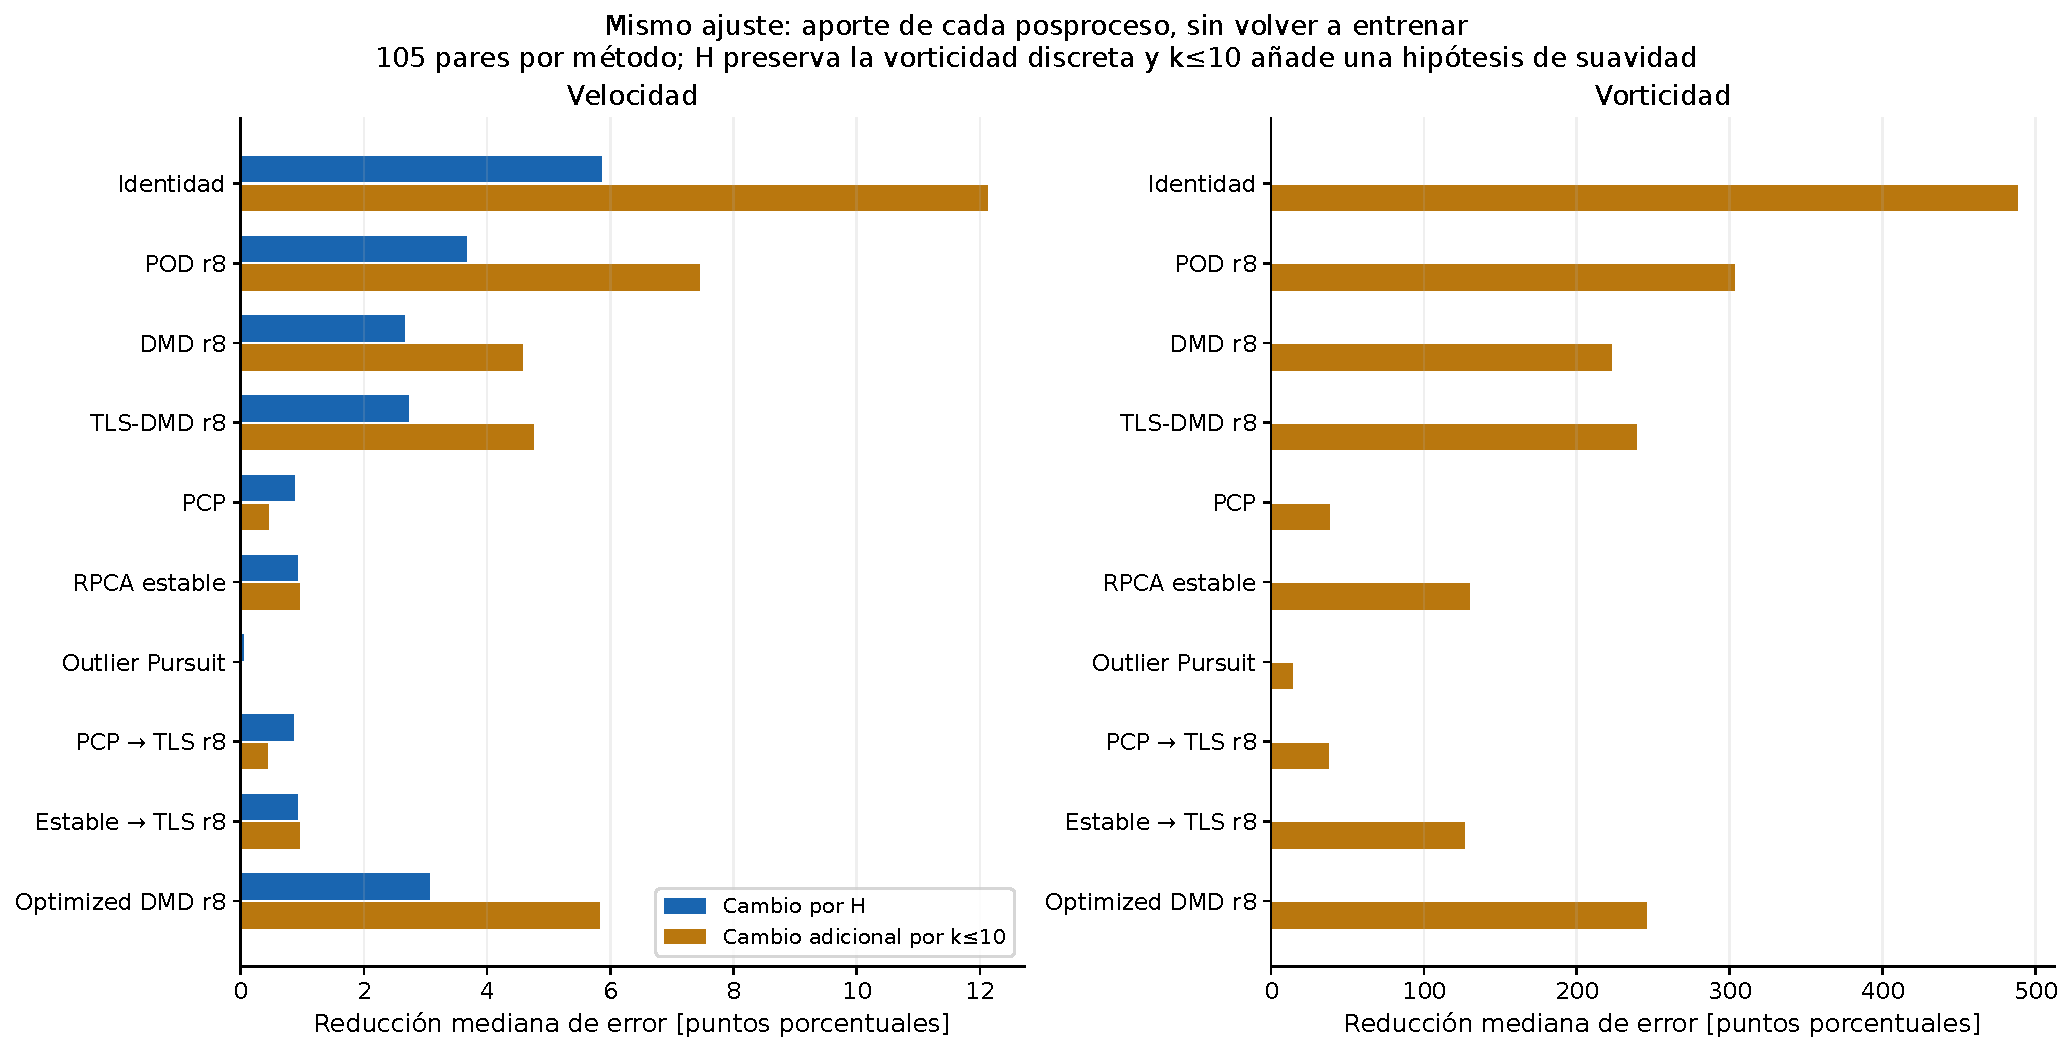
\includegraphics[width=\linewidth,height=.80\textwidth,keepaspectratio]{results/research/model_fidelity_benchmark_2026-10-14/figures/prior_contributions.pdf}
\caption{Aportes pareados de imponer divergencia y limitar banda física. Cada transición compara el mismo ajuste y la misma contaminación. El control directo identity ayuda a atribuir la ganancia al estimador, al prior espacial o a su combinación, mientras los tres estados de aceptación conservan sus denominadores.}
\label{fig:paired-priors}\end{figure}
\end{landscape}
\clearpage

\clearpage
\begin{landscape}
\begin{figure}[p]\centering
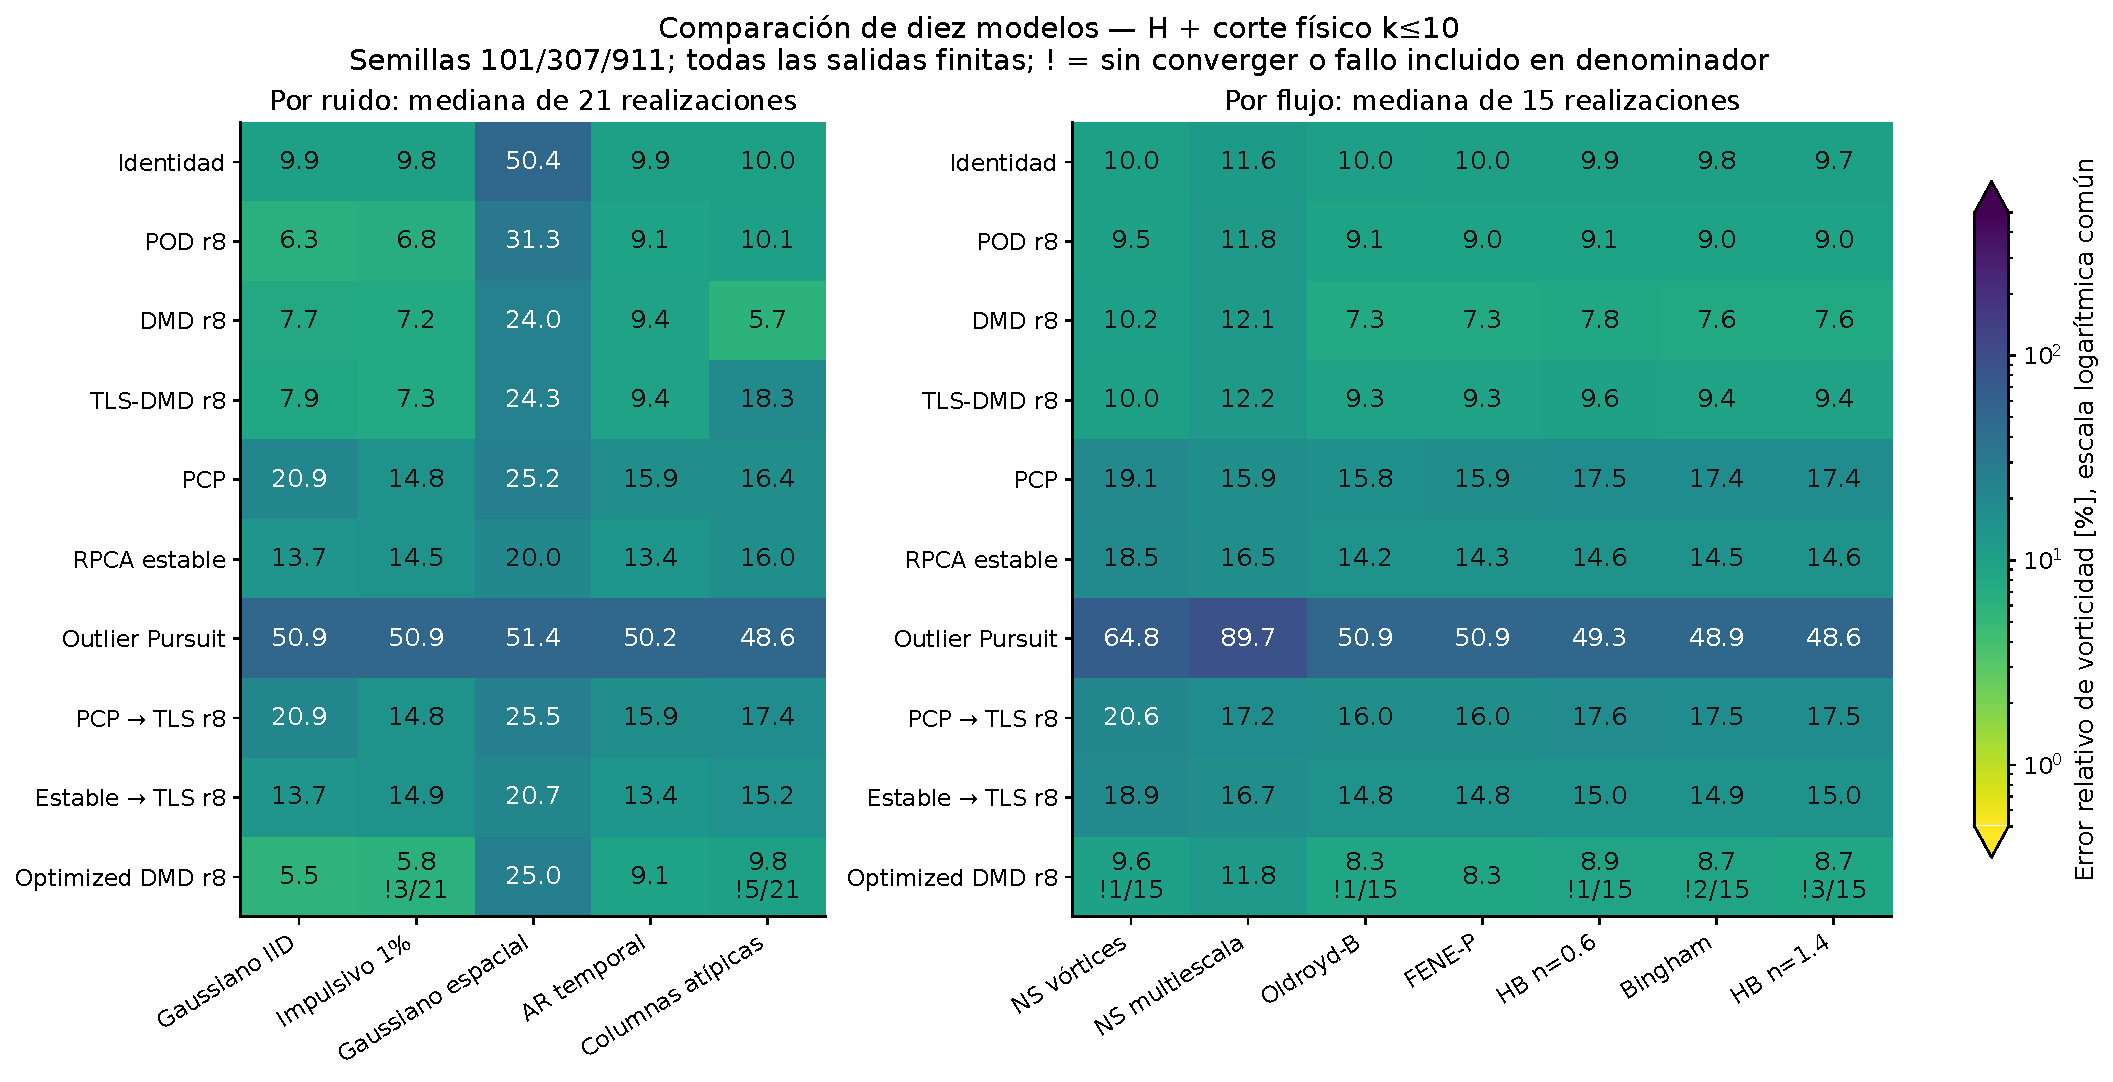
\includegraphics[width=\linewidth,height=.80\textwidth,keepaspectratio]{results/research/model_fidelity_benchmark_2026-10-14/figures/model_filtered_overview.pdf}
\caption{Comparación con idéntica proyección y banda física fija. El prior espacial se aplica también a identity; por ello una mejora frente a Raw no se atribuye enteramente a DMD o RPCA. Los errores que persisten identifican límites de la combinación de observación, modelo y conocimiento físico.}
\label{fig:models-common-prior}\end{figure}
\end{landscape}
\clearpage

\clearpage
\begin{landscape}
\begin{figure}[p]\centering
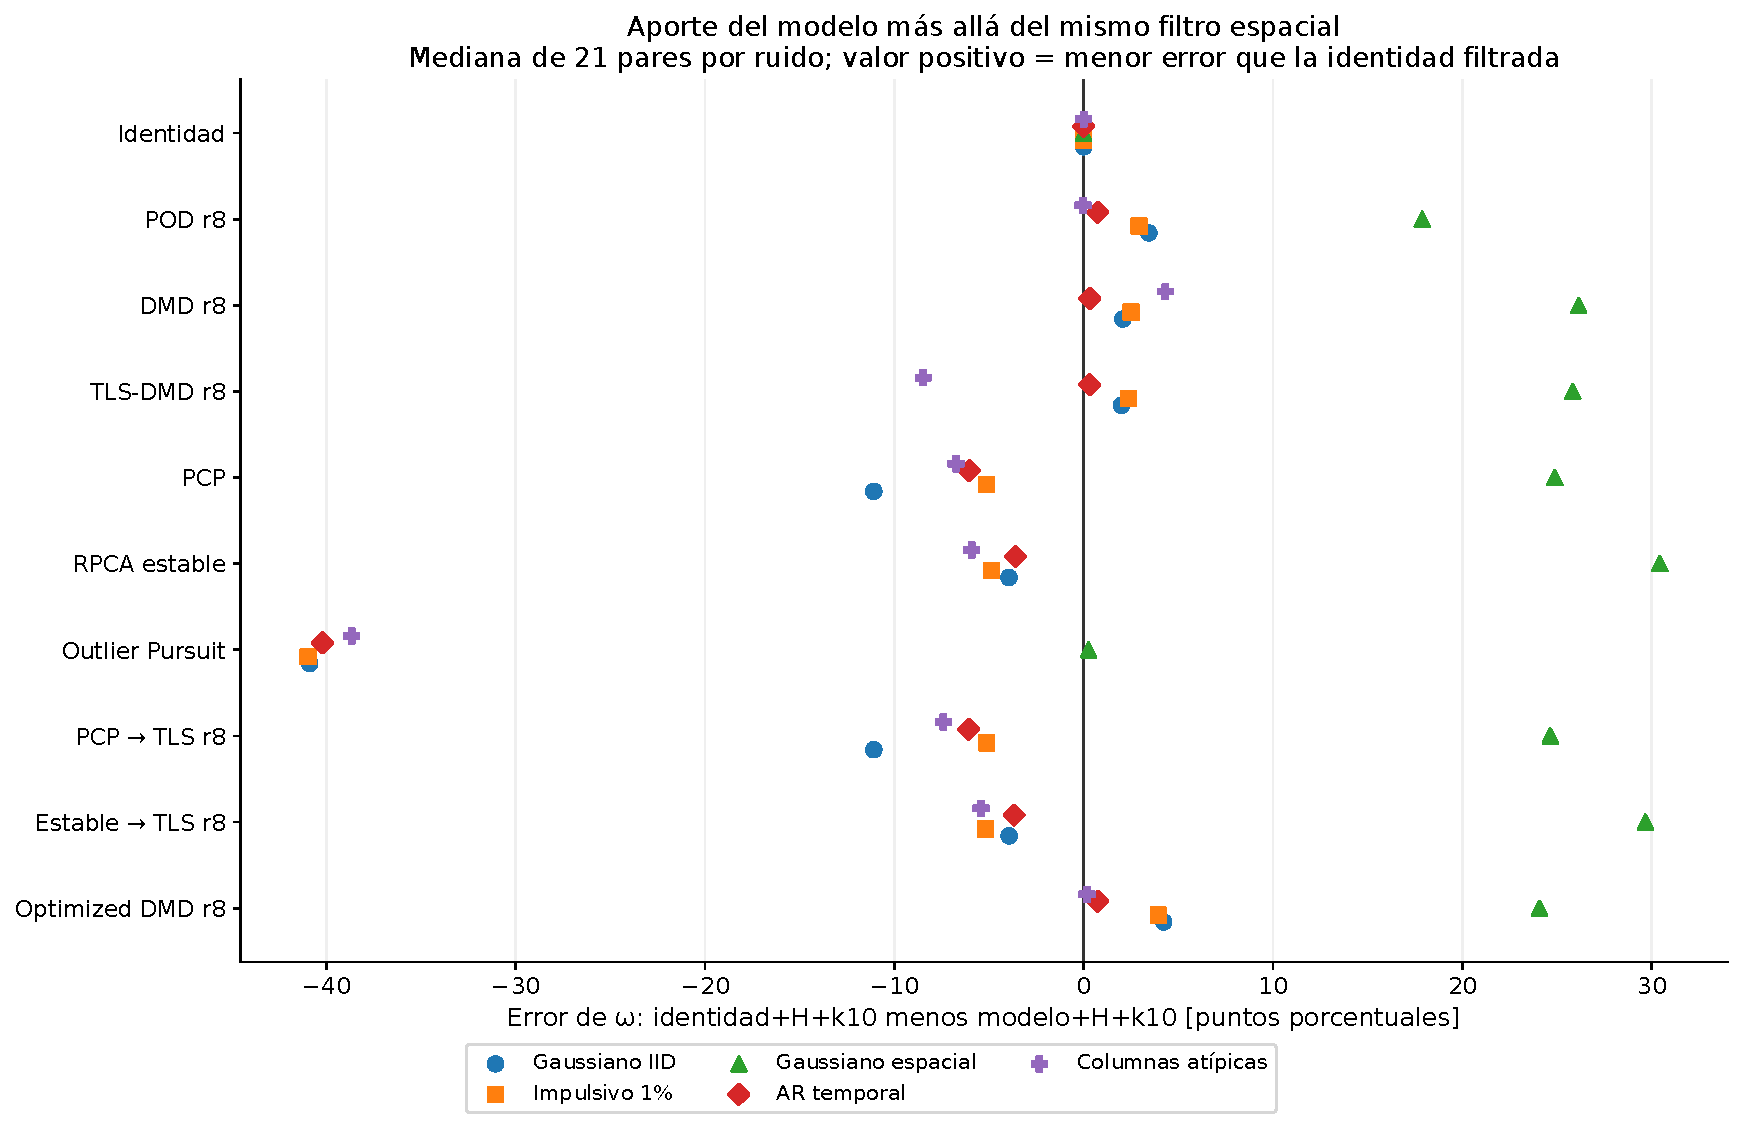
\includegraphics[width=\linewidth,height=.80\textwidth,keepaspectratio]{results/research/model_fidelity_benchmark_2026-10-14/figures/model_vs_identity.pdf}
\caption{Aporte del estimador frente al control directo sobre la misma observación y con el mismo posprocesamiento. Una ventaja de vorticidad requiere superar ese control físico; aceptar una salida y mejorar una métrica son criterios diferentes. Se conserva el emparejamiento por caso, ruido y semilla.}
\label{fig:model-control}\end{figure}
\end{landscape}
\clearpage

\subsection{Fidelidad que el prior elimina incluso con observación limpia}

\begingroup\small\setlength{\tabcolsep}{3pt}
\begin{longtable}{@{}>{\raggedright\arraybackslash}p{4.0cm}>{\raggedright\arraybackslash}p{2.2cm}>{\raggedright\arraybackslash}p{4.2cm}>{\raggedright\arraybackslash}p{4.2cm}@{}}
\caption{Pérdida de señal limpia por el prior k\_c=10 ya fijado. La referencia original completa sigue siendo el objetivo de fidelidad: no se cambia por una verdad filtrada más fácil de recuperar.}\\
\toprule
\textbf{Referencia 128$^2$} & \textbf{Corte físico} & \textbf{Señal perdida $e_u$} & \textbf{Señal perdida $e_\omega$} \\
\midrule\endfirsthead
\toprule
\textbf{Referencia 128$^2$} & \textbf{Corte físico} & \textbf{Señal perdida $e_u$} & \textbf{Señal perdida $e_\omega$} \\
\midrule\endhead
Vórtices NS & 10 & 0.461~\% & 3.541~\% \\
Multiescala NS & 10 & 3.068~\% & 10.84~\% \\
Oldroyd-B & 10 & 0.1671~\% & 1.448~\% \\
FENE-P & 10 & 0.1388~\% & 1.19~\% \\
HB n=0.6 & 10 & 0.2556~\% & 2.012~\% \\
Bingham & 10 & 0.1325~\% & 1.072~\% \\
HB n=1.4 & 10 & 0.08295~\% & 0.7561~\% \\
\bottomrule\end{longtable}\endgroup

El piso de vorticidad de una estimación limitada a esa banda es la norma de vorticidad limpia que queda fuera de la banda. El error restante proviene de reconstruir la parte retenida. Para identity H+B, Parseval separa exactamente pérdida de señal y ruido retenido en el error cuadrático, sin suponer independencia estadística entre ambos: sus soportes espectrales son ortogonales. Para otro estimador, la parte retenida incluye también su error de modelado y no se etiqueta únicamente como ruido.

\clearpage
\begin{landscape}
\begin{figure}[p]\centering
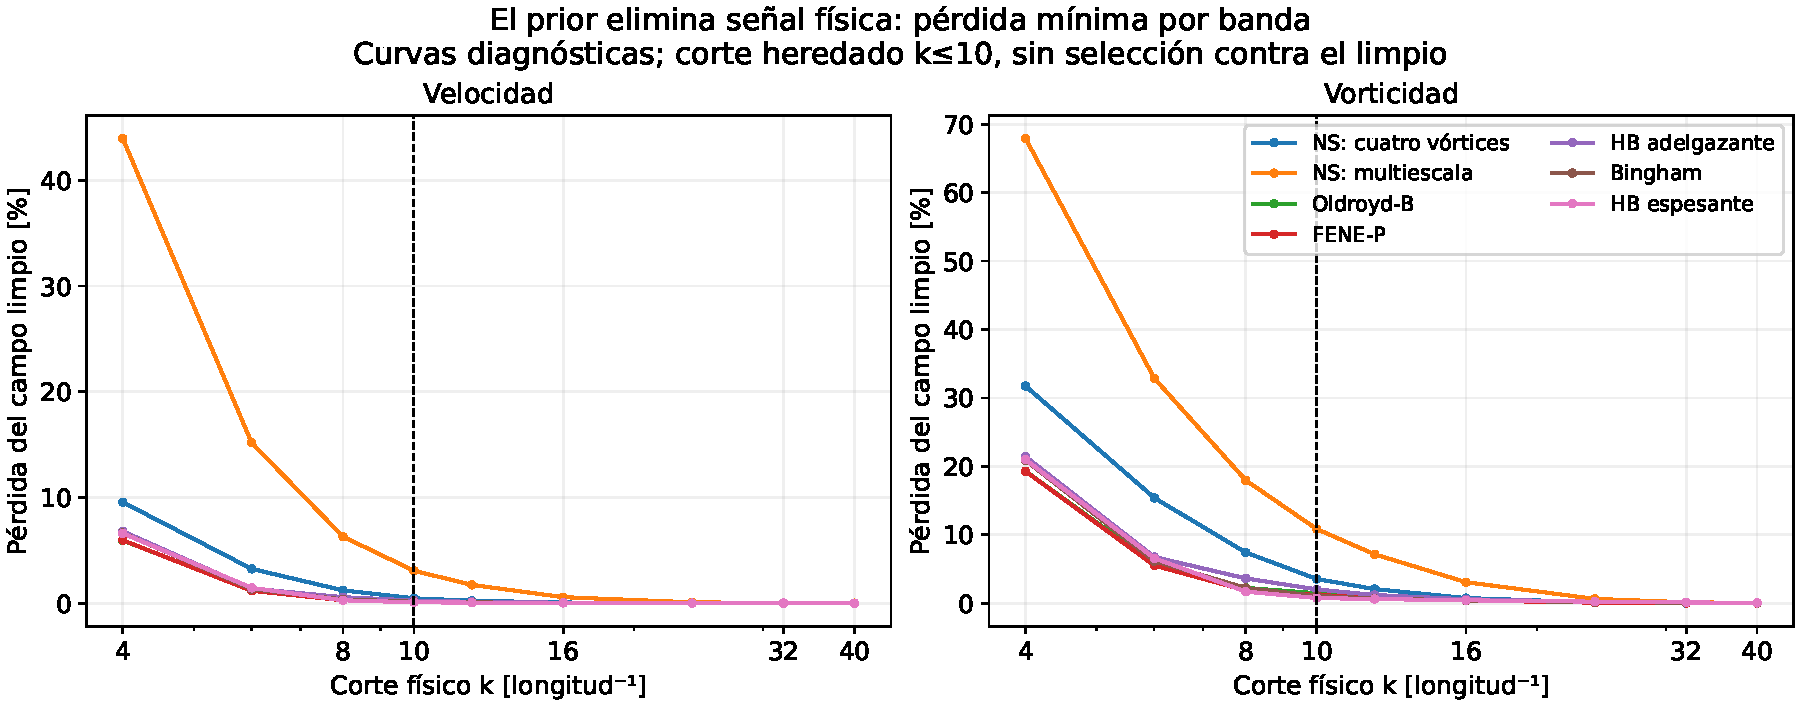
\includegraphics[width=\linewidth,height=.80\textwidth,keepaspectratio]{results/research/prior_spectral_budget_2026-10-14/figures/clean_bandwidth_bias.pdf}
\caption{Pérdida de estructura física con distintos cortes espaciales. Las curvas describen la referencia limpia y el corte k\_c=10 utilizado en la campaña permanece fijado. No se selecciona un nuevo corte minimizando error contra limpio; el diagnóstico muestra el costo de aceptar ese prior.}
\label{fig:clean-prior-bias}\end{figure}
\end{landscape}
\clearpage

\clearpage
\begin{landscape}
\begin{figure}[p]\centering
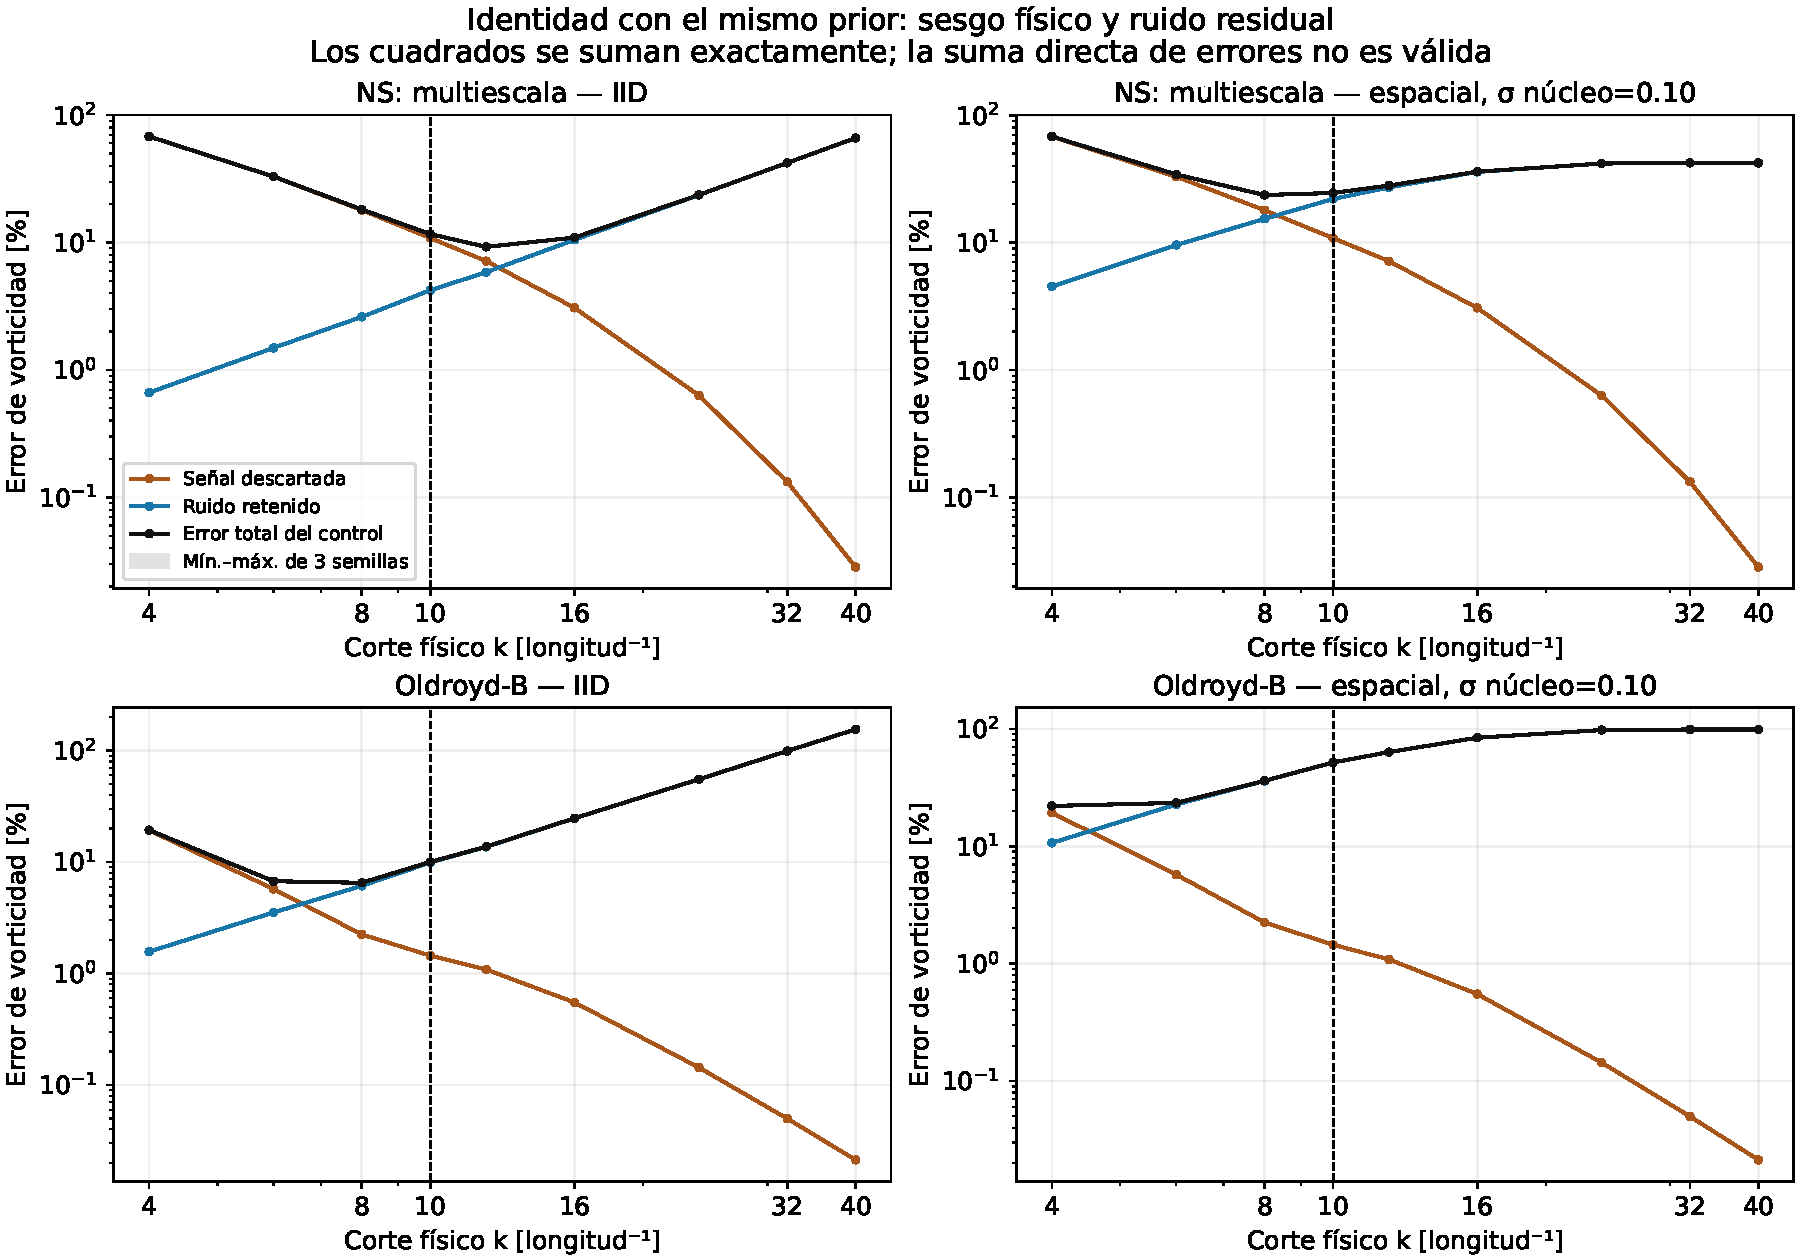
\includegraphics[width=\linewidth,height=.80\textwidth,keepaspectratio]{results/research/prior_spectral_budget_2026-10-14/figures/identity_bias_noise_tradeoff.pdf}
\caption{Descomposición del error de identity con proyección y banda fija: pérdida de señal fuera de banda y ruido proyectado que permanece dentro. La identidad sirve como control espacial del aporte del estimador. Las realizaciones son descriptivas y el error se mide contra todas las escalas de la referencia.}
\label{fig:prior-noise-budget}\end{figure}
\end{landscape}
\clearpage

\clearpage
\begin{landscape}
\begin{figure}[p]\centering
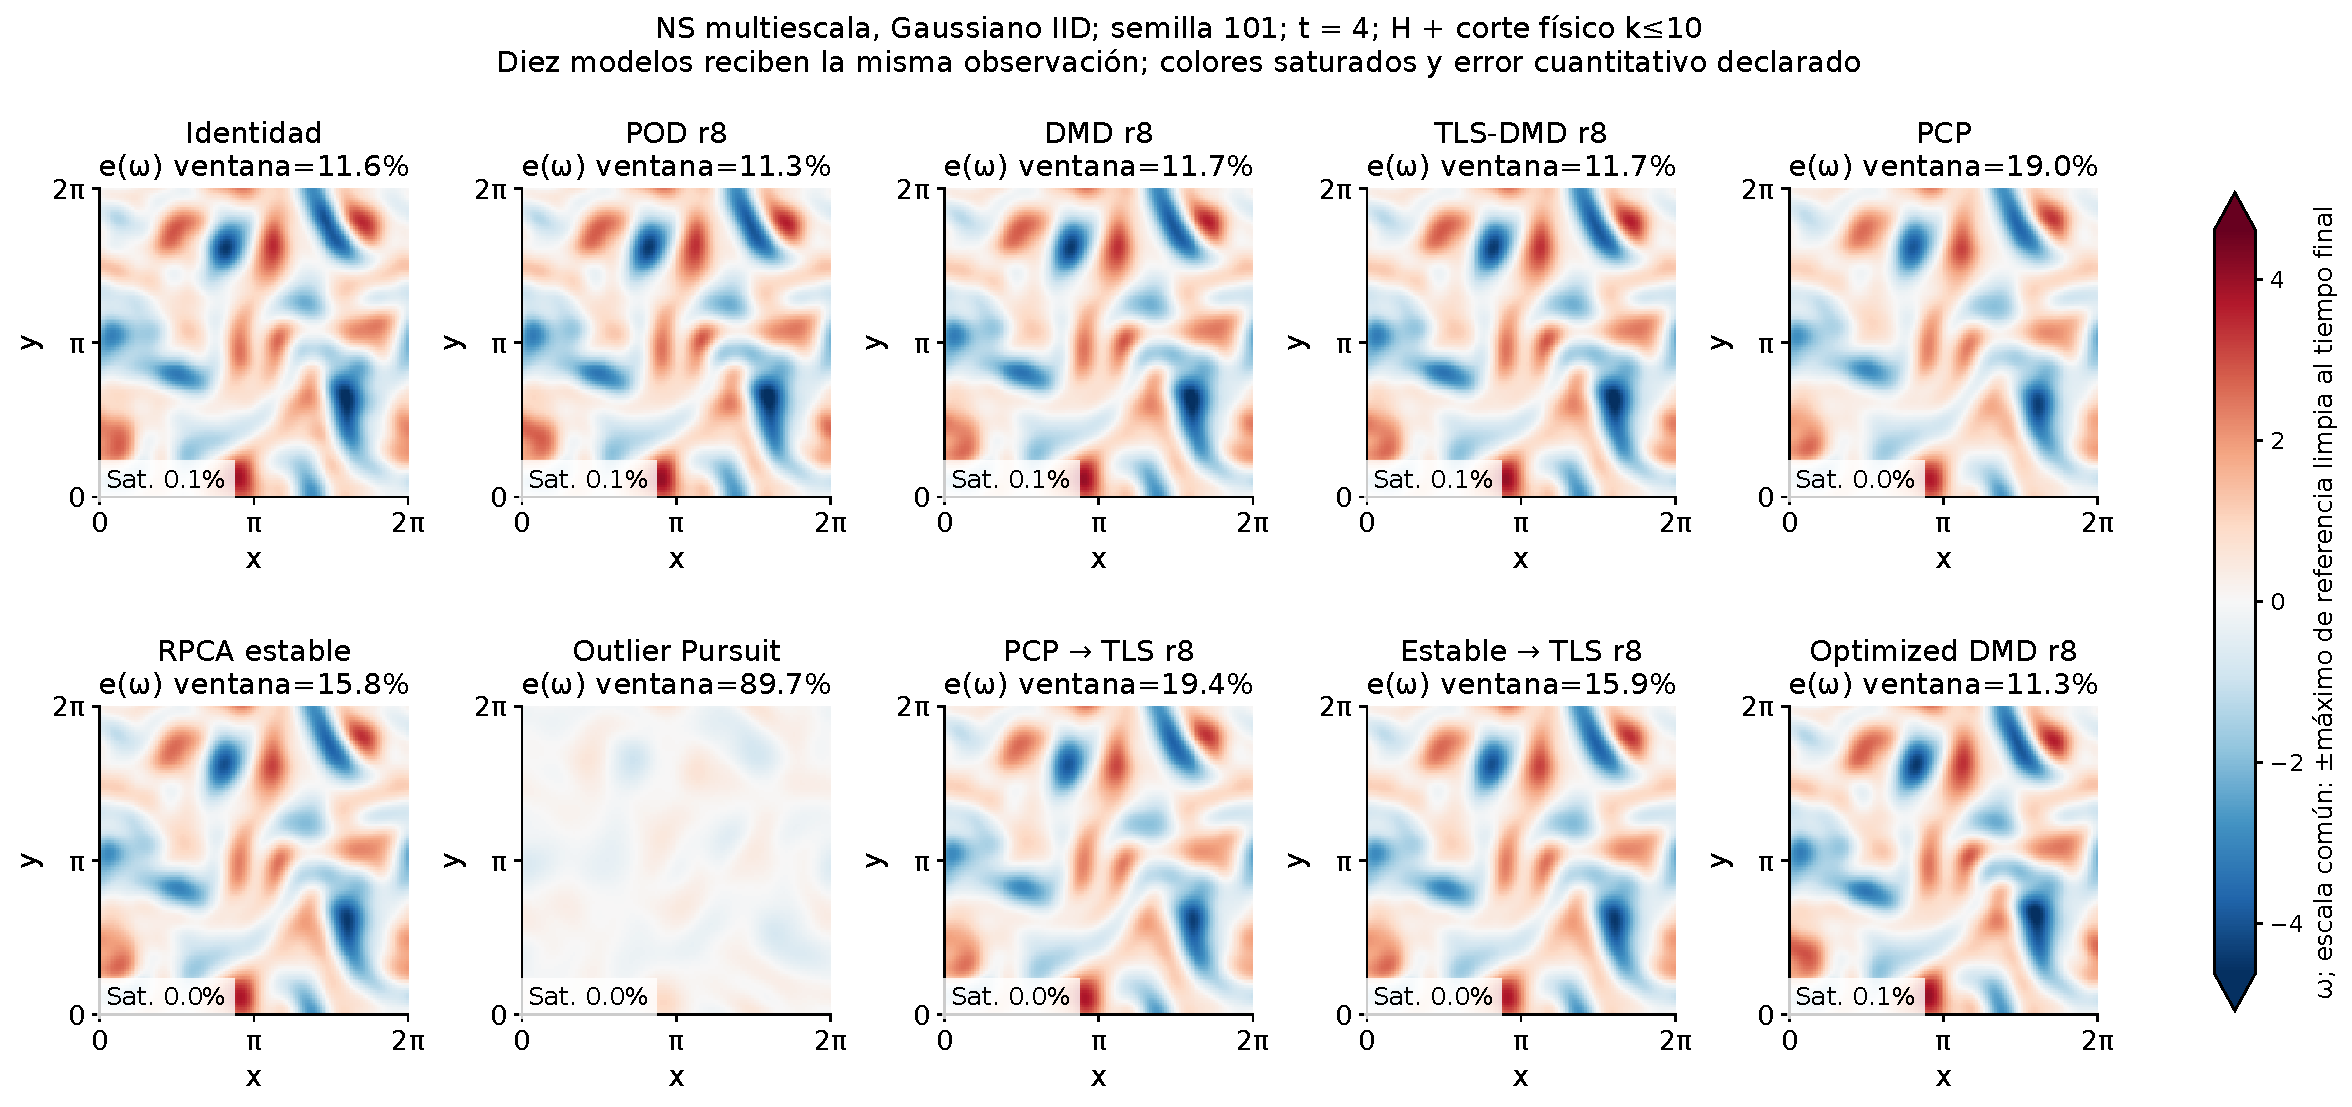
\includegraphics[width=\linewidth,height=.80\textwidth,keepaspectratio]{results/research/model_fidelity_benchmark_2026-10-14/figures/model_snapshots_ns_multiscale_gaussian_iid_helmholtz_k10.pdf}
\caption{Inspección espacial de las reconstrucciones multiescala con conocimiento físico común. Cada panel procede de un campo calculado; las escalas físicas y de diferencia se mantienen explícitas. El parecido visual se contrasta con los errores de campo completo y la aceptación, sin reemplazarlos.}
\label{fig:model-spatial-fidelity}\end{figure}
\end{landscape}
\clearpage

\clearpage
\section{Ruido, referencia física y costo a fidelidad exigida}

\begingroup\small\setlength{\tabcolsep}{3pt}
\begin{longtable}{@{}>{\raggedright\arraybackslash}p{4.0cm}>{\raggedright\arraybackslash}p{2.5cm}>{\raggedright\arraybackslash}p{2.5cm}>{\raggedright\arraybackslash}p{2.7cm}>{\raggedright\arraybackslash}p{2.7cm}@{}}
\caption{Cobertura por contaminación: una observación tiene solución cuando al menos una opción fija satisface convergencia y las cuatro puertas físicas. La última columna es un control fijo, no un ganador seleccionado con limpio.}\\
\toprule
\textbf{Contaminación} & \textbf{Con solución Raw} & \textbf{Con solución H} & \textbf{Con solución H+B} & \textbf{Identity H+B $e_\omega$} \\
\midrule\endfirsthead
\toprule
\textbf{Contaminación} & \textbf{Con solución Raw} & \textbf{Con solución H} & \textbf{Con solución H+B} & \textbf{Identity H+B $e_\omega$} \\
\midrule\endhead
Gaussiano IID & 0/21 & 0/21 & 21/21 & 9.937~\% \\
Impulsivo disperso & 3/21 & 12/21 & 21/21 & 9.844~\% \\
Espacial correlacionado & 0/21 & 3/21 & 21/21 & 50.42~\% \\
Temporal AR & 0/21 & 0/21 & 21/21 & 9.879~\% \\
Columnas corruptas & 0/21 & 1/21 & 21/21 & 9.963~\% \\
\bottomrule\end{longtable}\endgroup

RMS igual controla energía inyectada, no dificultad de las derivadas. El ruido IID concentra parte de esa energía en frecuencias altas; el ruido espacial correlacionado solapa estructuras suaves de la señal. La memoria AR puede parecer dinámica modal y la corrupción de columnas elimina información temporal completa. Las conclusiones se apoyan en estas cinco contaminaciones y en sus parámetros, no en todo sensor real posible.

\begingroup\small\setlength{\tabcolsep}{3pt}
\begin{longtable}{@{}>{\raggedright\arraybackslash}p{3.7cm}>{\raggedright\arraybackslash}p{2.2cm}>{\raggedright\arraybackslash}p{2.2cm}>{\raggedright\arraybackslash}p{2.2cm}>{\raggedright\arraybackslash}p{2.2cm}>{\raggedright\arraybackslash}p{2.1cm}@{}}
\caption{Comparación centrada en RPCA y DMD: mediana de $e_\omega$ de salidas finitas entre siete referencias y tres semillas para cada ruido. No hay elección retrospectiva de hiperparámetro o ganador; las opciones son fijas y las condiciones siguen emparejadas.}\\
\toprule
\textbf{Contaminación} & \textbf{PCP Raw} & \textbf{DMD Raw} & \textbf{TLS Raw} & \textbf{TLS H+B} & \textbf{Identity H+B} \\
\midrule\endfirsthead
\toprule
\textbf{Contaminación} & \textbf{PCP Raw} & \textbf{DMD Raw} & \textbf{TLS Raw} & \textbf{TLS H+B} & \textbf{Identity H+B} \\
\midrule\endhead
Gaussiano IID & 167.3~\% & 249.2~\% & 249.5~\% & 7.86~\% & 9.937~\% \\
Impulsivo disperso & 22.62~\% & 228.2~\% & 228.7~\% & 7.322~\% & 9.844~\% \\
Espacial correlacionado & 62.85~\% & 43.9~\% & 44.31~\% & 24.3~\% & 50.42~\% \\
Temporal AR & 353.7~\% & 464.4~\% & 464.3~\% & 9.436~\% & 9.879~\% \\
Columnas corruptas & 47.67~\% & 239.7~\% & 655.3~\% & 18.3~\% & 9.963~\% \\
\bottomrule\end{longtable}\endgroup

\begingroup\small\setlength{\tabcolsep}{3pt}
\begin{longtable}{@{}>{\raggedright\arraybackslash}p{3.3cm}>{\raggedright\arraybackslash}p{2.4cm}>{\raggedright\arraybackslash}p{2.4cm}>{\raggedright\arraybackslash}p{3.0cm}>{\raggedright\arraybackslash}p{1.8cm}>{\raggedright\arraybackslash}p{1.7cm}@{}}
\caption{Contraste pareado fijo de RPCA/PCP y TLS-DMD sin prior físico, en puntos porcentuales. Valores negativos favorecen PCP. Se usan diagnósticos finitos aun si no convergen, identificados en la última columna; la aceptación se exige por separado.}\\
\toprule
\textbf{Contaminación} & \textbf{$\Delta$ $e_u$ PCP-TLS} & \textbf{$\Delta$ $e_\omega$ PCP-TLS} & \textbf{PCP gana / empata / pierde $\omega$} & \textbf{Pares finitos} & \textbf{No conv. en par} \\
\midrule\endfirsthead
\toprule
\textbf{Contaminación} & \textbf{$\Delta$ $e_u$ PCP-TLS} & \textbf{$\Delta$ $e_\omega$ PCP-TLS} & \textbf{PCP gana / empata / pierde $\omega$} & \textbf{Pares finitos} & \textbf{No conv. en par} \\
\midrule\endhead
Gaussiano IID & 2.981 pp & -83.14 pp & 21/0/0 & 21/21 & 0 \\
Impulsivo disperso & -2.56 pp & -203.2 pp & 21/0/0 & 21/21 & 0 \\
Espacial correlacionado & 3.723 pp & 16.91 pp & 0/0/21 & 21/21 & 0 \\
Temporal AR & -2.353 pp & -106.3 pp & 21/0/0 & 21/21 & 0 \\
Columnas corruptas & -17.17 pp & -602.8 pp & 21/0/0 & 21/21 & 0 \\
\bottomrule\end{longtable}\endgroup

\subsection{Del campo de velocidad a la fidelidad física}

\begingroup\small\setlength{\tabcolsep}{3pt}
\begin{longtable}{@{}>{\raggedright\arraybackslash}p{2.9717cm}>{\raggedright\arraybackslash}p{4.2594cm}>{\raggedright\arraybackslash}p{2.2783cm}>{\raggedright\arraybackslash}p{2.7736cm}>{\raggedright\arraybackslash}p{2.7736cm}@{}}
\caption{Diagnóstico viscoplástico condicionado a la constitutiva conocida: medianas sobre cinco ruidos y tres semillas. La norma de esfuerzo simétrico incluye dos veces la componente cortante; no es la norma de un vector de tres componentes.}\\
\toprule
\textbf{Fluido} & \textbf{Estimador H+B} & \textbf{$e_\omega$} & \textbf{e\_esfuerzo} & \textbf{e\_viscosidad} \\
\midrule\endfirsthead
\toprule
\textbf{Fluido} & \textbf{Estimador H+B} & \textbf{$e_\omega$} & \textbf{e\_esfuerzo} & \textbf{e\_viscosidad} \\
\midrule\endhead
HB n=0.6 & Identity & 9.879~\% & 12.57~\% & 18.49~\% \\
HB n=0.6 & TLS-DMD r=8 & 9.57~\% & 11.94~\% & 17.78~\% \\
HB n=0.6 & RPCA/PCP & 17.54~\% & 15.24~\% & 18.56~\% \\
HB n=0.6 & RPCA estable & 14.58~\% & 13.06~\% & 17.19~\% \\
Bingham & Identity & 9.761~\% & 10.51~\% & 8.337~\% \\
Bingham & TLS-DMD r=8 & 9.436~\% & 10.08~\% & 7.837~\% \\
Bingham & RPCA/PCP & 17.42~\% & 16.33~\% & 8.406~\% \\
Bingham & RPCA estable & 14.5~\% & 13.68~\% & 7.863~\% \\
HB n=1.4 & Identity & 9.744~\% & 9.673~\% & 8.136~\% \\
HB n=1.4 & TLS-DMD r=8 & 9.418~\% & 9.401~\% & 7.64~\% \\
HB n=1.4 & RPCA/PCP & 17.45~\% & 18.86~\% & 8.046~\% \\
HB n=1.4 & RPCA estable & 14.59~\% & 15.59~\% & 7.58~\% \\
\bottomrule\end{longtable}\endgroup

El esfuerzo y la viscosidad viscoplásticos se derivan del gradiente reconstruido y de parámetros materiales conocidos, sin copiar el esfuerzo limpio. Su error puede diferir del de vorticidad porque la ley de viscosidad es no lineal y sensible a corte pequeño. En Oldroyd-B/FENE-P el esfuerzo depende de la memoria de conformación y no queda identificado por velocidad sola; se informa como no disponible. Esas ausencias no se convierten en ceros.

Una serie de energía próxima a la referencia no demuestra por sí sola su balance dinámico. La disipación integra gradientes y la ley constitutiva, mientras el balance relaciona esa disipación con la derivada temporal de energía. El banco informa el error de disipación cuando es identificable y mantiene separados esos diagnósticos de la aceptación operacional. La masa total con densidad fija es un control trivial; la continuidad local y la evolución del campo contienen información adicional.

\clearpage
\begin{landscape}
\begin{figure}[p]\centering
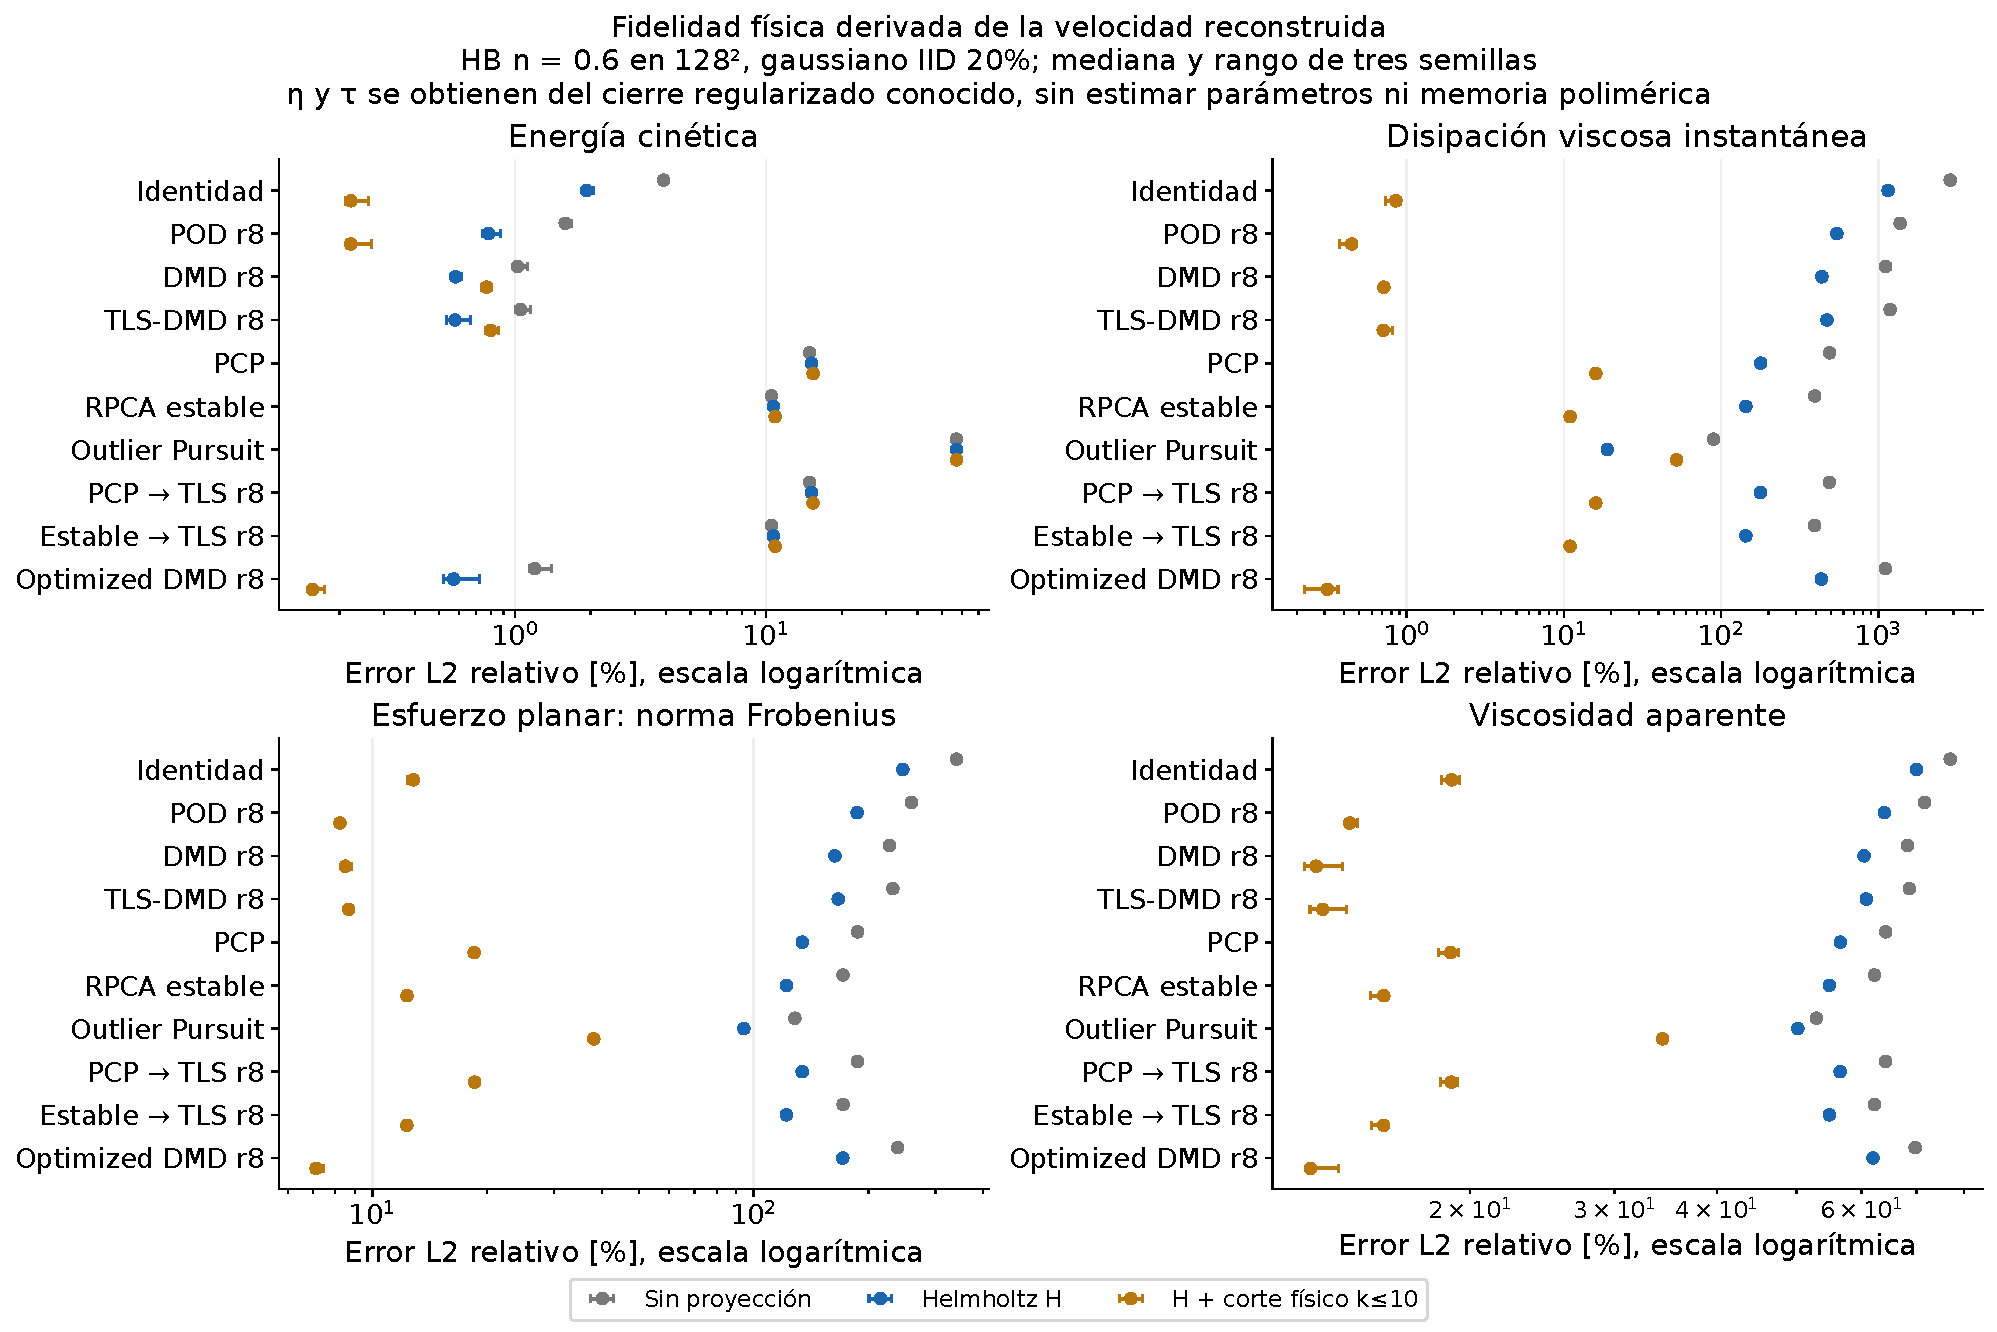
\includegraphics[width=\linewidth,height=.80\textwidth,keepaspectratio]{results/research/model_fidelity_benchmark_2026-10-14/figures/constitutive_fidelity_hb_thinning_gaussian_iid.pdf}
\caption{Fidelidad física adicional en HB adelgazante con ruido gaussiano IID: energía, disipación viscosa, esfuerzo de Frobenius y viscosidad aparente bajo Raw/H/H+B. Las medianas y extremos representan tres realizaciones del mismo caso. El cierre material conocido se aplica al gradiente reconstruido y no identifica parámetros ni certifica la ecuación de movimiento.}
\label{fig:constitutive-reconstruction-fidelity}\end{figure}
\end{landscape}
\clearpage

\clearpage
\begin{landscape}
\begin{figure}[p]\centering
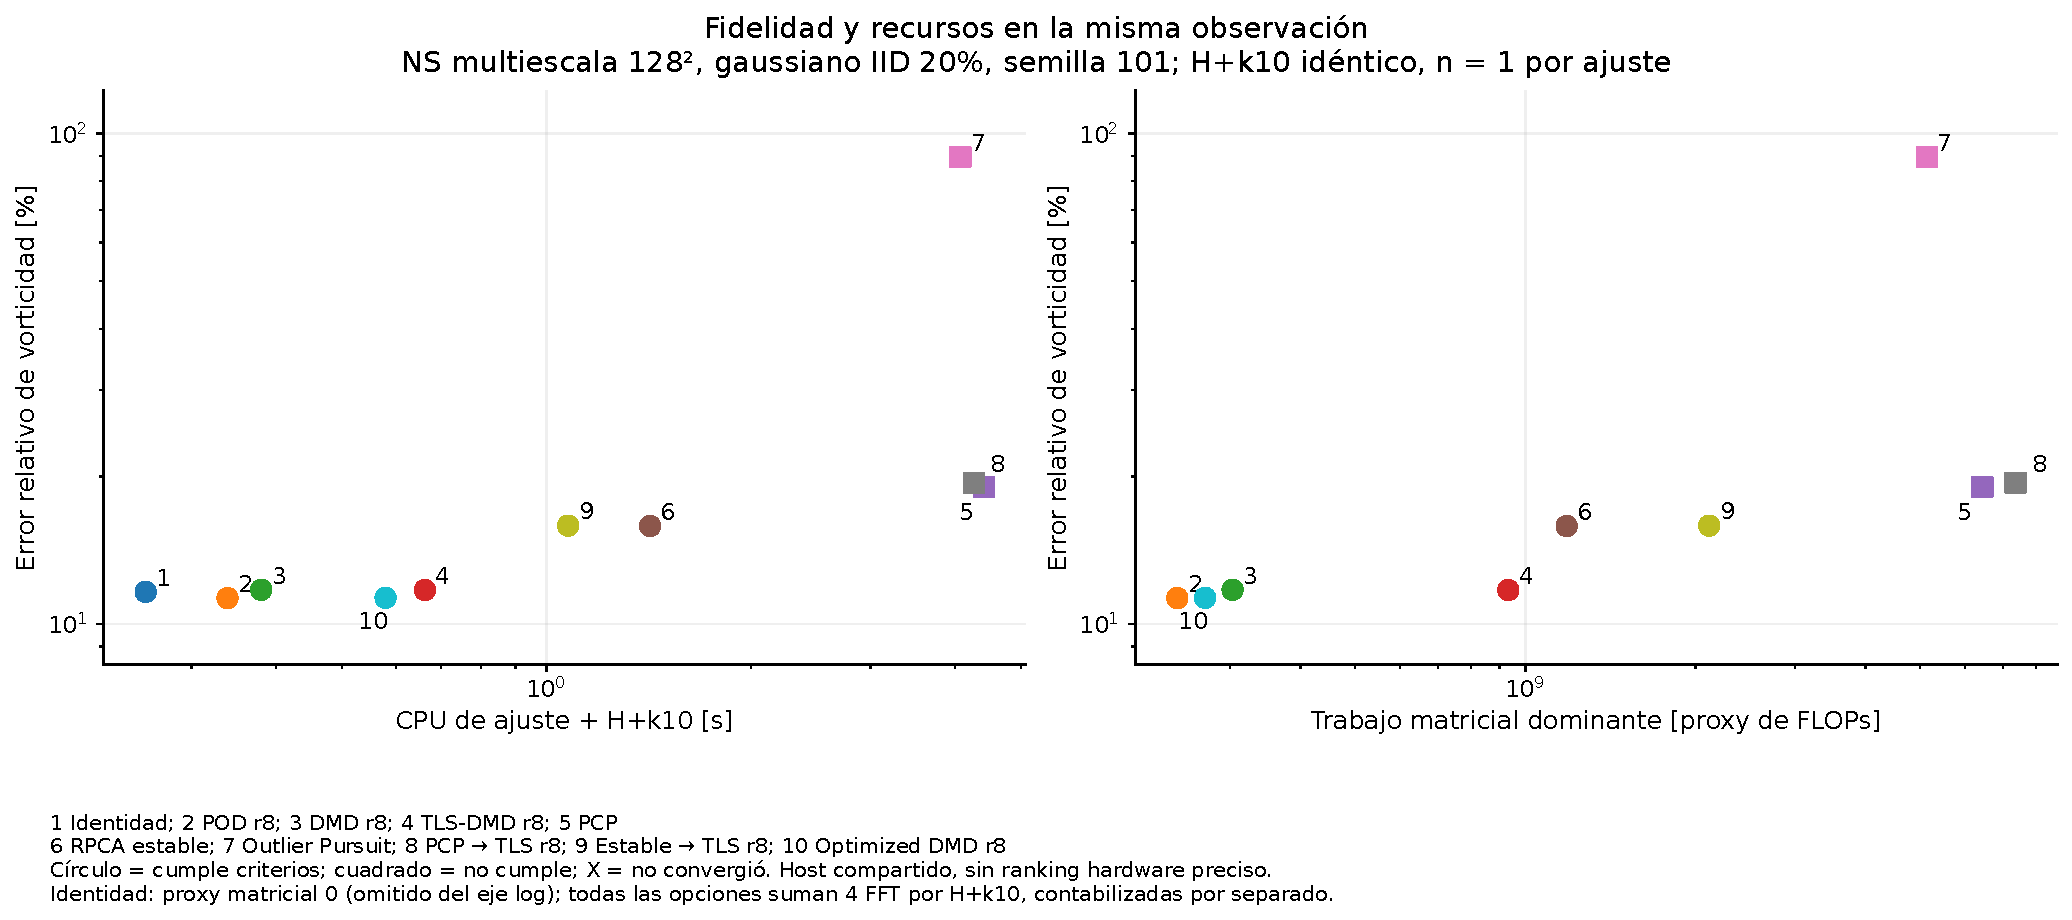
\includegraphics[width=\linewidth,height=.80\textwidth,keepaspectratio]{results/research/model_fidelity_benchmark_2026-10-14/figures/cost_fidelity.pdf}
\caption{Recursos y fidelidad en una misma observación Multiescala NS, ruido gaussiano IID y semilla 101, con H+B. El costo suma ajuste y esta variante de posprocesamiento. La admisibilidad exige las cuatro puertas y convergencia, además de un error de velocidad pequeño. Las mediciones de este banco tienen una réplica por ajuste en el host declarado: describen ese entorno y no justifican diferencias finas de rendimiento ni memoria incremental exclusiva.}
\label{fig:cost-at-fidelity}\end{figure}
\end{landscape}
\clearpage

\begingroup\small\setlength{\tabcolsep}{3pt}
\begin{longtable}{@{}>{\raggedright\arraybackslash}p{4.2041cm}>{\raggedright\arraybackslash}p{2.3465cm}>{\raggedright\arraybackslash}p{3.1286cm}>{\raggedright\arraybackslash}p{2.4442cm}>{\raggedright\arraybackslash}p{2.9331cm}@{}}
\caption{Comparación de recursos en el mismo bloque de la figura. La CPU suma ajuste y su posprocesamiento; la RSS es pico absoluto del ajuste y el trabajo FFT se informa aparte del proxy matricial. ND indica dato no disponible.}\\
\toprule
\textbf{Estimador H+B} & \textbf{CPU cadena, s} & \textbf{Trabajo matricial proxy} & \textbf{RSS ajuste, MiB} & \textbf{Estado físico} \\
\midrule\endfirsthead
\toprule
\textbf{Estimador H+B} & \textbf{CPU cadena, s} & \textbf{Trabajo matricial proxy} & \textbf{RSS ajuste, MiB} & \textbf{Estado físico} \\
\midrule\endhead
Identity & 0.2569 & 0 & 152.2 & Admisible \\
POD r=8 & 0.3391 & 2.420e+08 & 173.5 & Admisible \\
DMD r=8 & 0.38 & 3.032e+08 & 174.4 & Admisible \\
TLS-DMD r=8 & 0.6622 & 9.326e+08 & 233 & Admisible \\
RPCA/PCP & 4.41 & 6.440e+09 & 225.3 & Fuera de puertas \\
RPCA estable & 1.421 & 1.183e+09 & 204.7 & Admisible \\
Outlier Pursuit & 4.071 & 5.139e+09 & 215.1 & Fuera de puertas \\
PCP + TLS-DMD & 4.26 & 7.372e+09 & 259.8 & Fuera de puertas \\
RPCA estable + TLS-DMD & 1.076 & 2.116e+09 & 244.9 & Admisible \\
Optimized DMD r=8 & 0.5795 & 2.711e+08 & 173.3 & Admisible \\
\bottomrule\end{longtable}\endgroup

La CPU, RSS absoluta y proxy de operaciones complementan el tiempo de pared. La memoria incluye intérprete y entrada; el proxy registra trabajo dominante aproximado, no FLOPs instrumentados ni energía eléctrica. El pico RSS del posprocesamiento hereda máximos previos del proceso, incluso de una evaluación anterior; se conserva separado de la memoria del ajuste y no se interpreta como memoria incremental de la proyección. La comparación de costo empieza por filtrar soluciones admisibles dentro del mismo bloque. Si no existe ninguna, el costo a la tolerancia queda sin solución, en vez de premiar al método más rápido que falla. El reanálisis histórico conserva tres mediciones por condición y permite revisar variabilidad de costo sin aumentar artificialmente el número de observaciones de calidad.

\clearpage
\section{Sensibilidad y límites de la comparación}

El estudio de sensibilidad registra 360 ajustes y 1080 salidas físicas, con 0 fallos y 0 ajustes no convergentes. Cambia rango e intensidad sobre Multiescala NS y Oldroyd-B en 128$^2$. Cruza r=2,4,8,12,16; intensidades RMS 5~\%, 20~\% y 40~\%; ruido gaussiano e impulsivo; POD y TLS-DMD; y las mismas tres semillas nuevas. El diseño fija los valores antes de ejecutar. Es un análisis exploratorio de configuraciones, sin escoger rango contra limpio para transferirlo a otra medición. Los puntos r=8 y 20~\% coincidentes con el banco principal no se cuentan como evidencia independiente.

La aceptación operacional es 0/360 con Raw, 12/360 con H y 324/360 con H+B. Estos conteos cruzan sólo POD y TLS-DMD, dos flujos y los valores de rango/intensidad declarados. La interpretación del aporte del filtro requiere el control identity del banco principal, que comparte el mismo prior.

\begingroup\small\setlength{\tabcolsep}{3pt}
\begin{longtable}{@{}>{\raggedright\arraybackslash}p{3.3cm}>{\raggedright\arraybackslash}p{1.3cm}>{\raggedright\arraybackslash}p{3.0cm}>{\raggedright\arraybackslash}p{3.0cm}>{\raggedright\arraybackslash}p{3.8cm}@{}}
\caption{Diagnóstico del sesgo de compresión y filtrado. La SVD limpia minimiza Frobenius de velocidad a rango fijado; su error de vorticidad es diagnóstico y no un óptimo universal. La banda física elimina también señal real.}\\
\toprule
\textbf{Referencia} & \textbf{Rango} & \textbf{POD limpio $e_u$} & \textbf{POD limpio $e_\omega$} & \textbf{Banda limpia $e_\omega$} \\
\midrule\endfirsthead
\toprule
\textbf{Referencia} & \textbf{Rango} & \textbf{POD limpio $e_u$} & \textbf{POD limpio $e_\omega$} & \textbf{Banda limpia $e_\omega$} \\
\midrule\endhead
Multiescala NS & 2 & 29.89~\% & 40.32~\% & 10.84~\% \\
Multiescala NS & 8 & 1.411~\% & 4.21~\% & 10.84~\% \\
Multiescala NS & 16 & 0.07647~\% & 0.3772~\% & 10.84~\% \\
Oldroyd-B & 2 & 9.283~\% & 19.04~\% & 1.448~\% \\
Oldroyd-B & 8 & 0.08052~\% & 0.5634~\% & 1.448~\% \\
Oldroyd-B & 16 & 0.002164~\% & 0.03689~\% & 1.448~\% \\
\bottomrule\end{longtable}\endgroup

El filtro no es gratuito: la pérdida de vorticidad limpia depende del caso, aunque se mantenga k\_c=10. La menor pérdida de una referencia frente a otra puede facilitar su aceptación con la misma puerta del 25~\%. POD de mayor rango aproxima mejor la velocidad limpia, pero en datos ruidosos puede retener más gradientes de contaminación. La curva de error observada, y no el rango óptimo del limpio, describe ese intercambio entre compresión y ruido.

\clearpage
\begin{landscape}
\begin{figure}[p]\centering
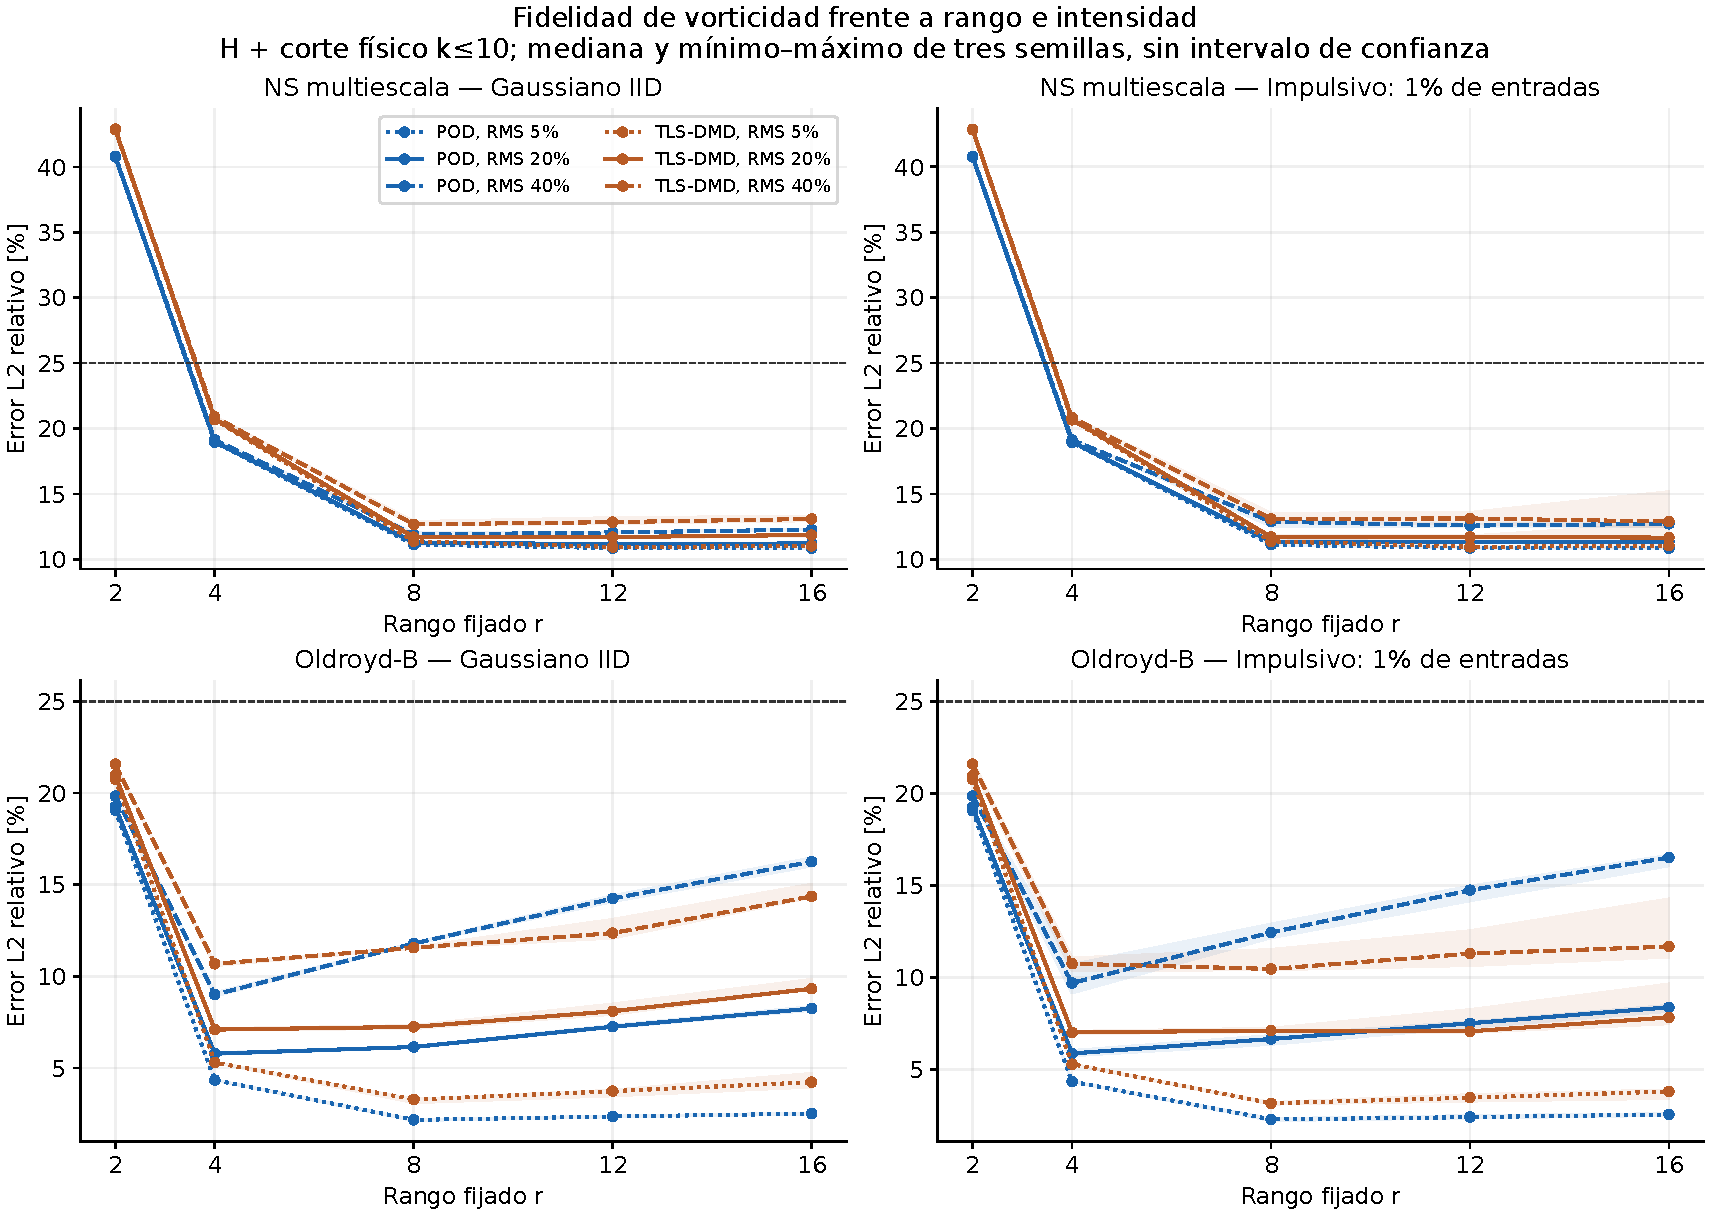
\includegraphics[width=\linewidth,height=.80\textwidth,keepaspectratio]{results/research/rank_noise_sensitivity_2026-10-14/figures/rank_vorticity.pdf}
\caption{Sensibilidad del error al rango y a la intensidad. Las bandas muestran mínimo y máximo de tres realizaciones de observación, no intervalos de confianza poblacionales. Aumentar rango puede recuperar señal omitida y también incorporar ruido; el comportamiento debe leerse junto con la vorticidad y el prior aplicado.}
\label{fig:rank-intensity}\end{figure}
\end{landscape}
\clearpage

\begingroup\small\setlength{\tabcolsep}{3pt}
\begin{longtable}{@{}>{\raggedright\arraybackslash}p{4.5cm}>{\raggedright\arraybackslash}p{2.4cm}>{\raggedright\arraybackslash}p{1.2cm}>{\raggedright\arraybackslash}p{2.1cm}>{\raggedright\arraybackslash}p{2.1cm}>{\raggedright\arraybackslash}p{2.1cm}@{}}
\caption{Ejemplos descriptivos de sensibilidad, medianas de tres semillas: aumentar rango puede aumentar vorticidad de ruido, y dos estimadores pueden intercambiar ventaja en velocidad y gradientes.}\\
\toprule
\textbf{Referencia y observación} & \textbf{Modelo} & \textbf{Rango} & \textbf{Raw $e_\omega$} & \textbf{H+B $e_u$} & \textbf{H+B $e_\omega$} \\
\midrule\endfirsthead
\toprule
\textbf{Referencia y observación} & \textbf{Modelo} & \textbf{Rango} & \textbf{Raw $e_\omega$} & \textbf{H+B $e_u$} & \textbf{H+B $e_\omega$} \\
\midrule\endhead
Multiescala NS, Gaussiano IID, RMS 20~\% & POD & 8 & 96.64~\% & 3.396~\% & 11.3~\% \\
Multiescala NS, Gaussiano IID, RMS 20~\% & POD & 16 & 137.9~\% & 3.361~\% & 11.22~\% \\
Oldroyd-B, Impulsivo disperso, RMS 40~\% & POD & 16 & 838.3~\% & 3.456~\% & 16.52~\% \\
Oldroyd-B, Impulsivo disperso, RMS 40~\% & TLS-DMD & 16 & 428.1~\% & 4.108~\% & 11.68~\% \\
\bottomrule\end{longtable}\endgroup

\clearpage
\begin{landscape}
\begin{figure}[p]\centering
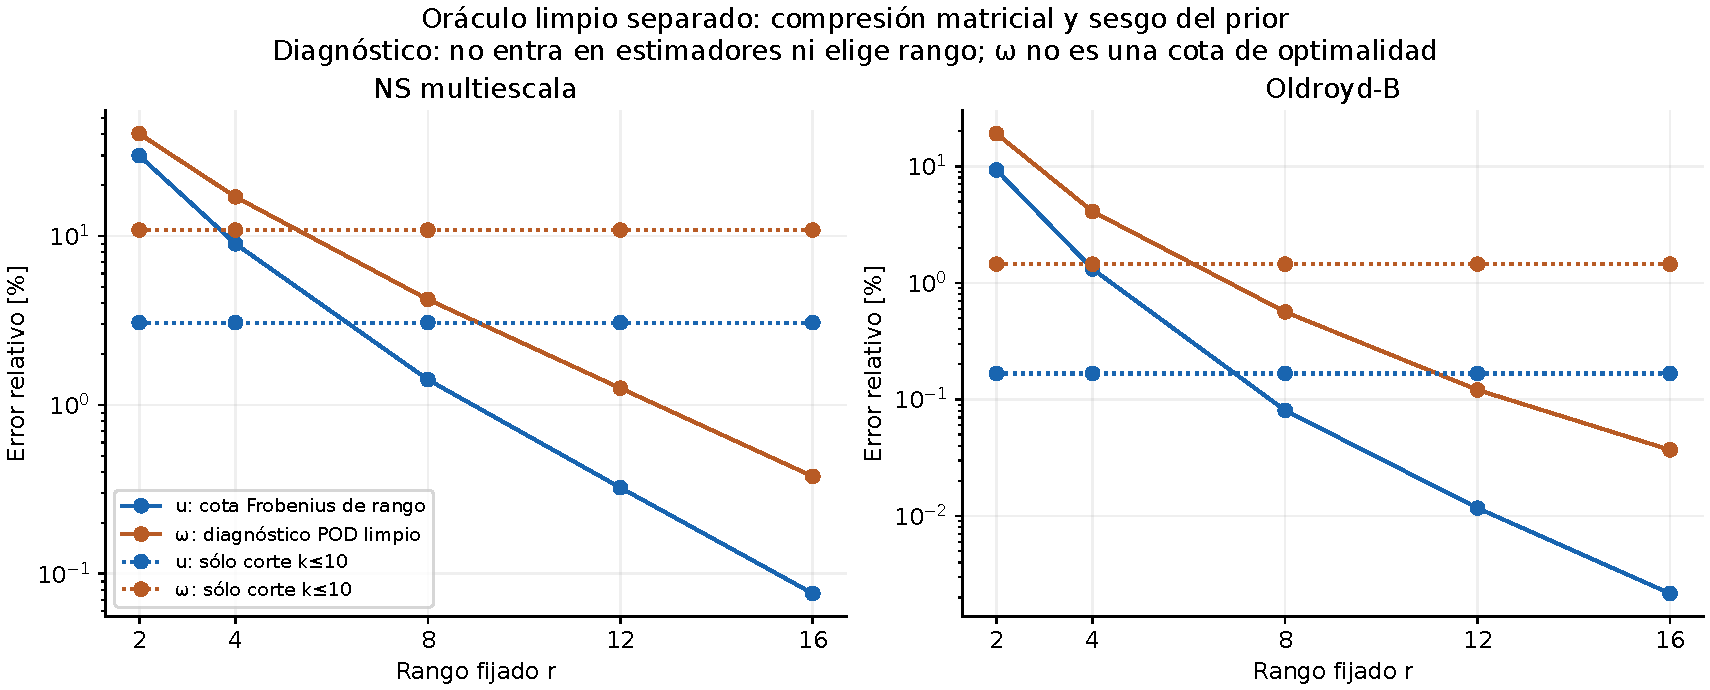
\includegraphics[width=\linewidth,height=.80\textwidth,keepaspectratio]{results/research/rank_noise_sensitivity_2026-10-14/figures/clean_oracle_floor.pdf}
\caption{Piso diagnóstico de compresión y filtrado del campo limpio. Este cálculo usa referencia sólo después del experimento para explicar sesgo de rango o banda; no interviene en entrenamiento ni selección. No es un método utilizable cuando la señal verdadera es desconocida.}
\label{fig:diagnostic-oracle}\end{figure}
\end{landscape}
\clearpage

\subsection{Qué conserva el reanálisis de las mallas pequeñas}

\begingroup\small\setlength{\tabcolsep}{3pt}
\begin{longtable}{@{}>{\raggedright\arraybackslash}p{4.2cm}>{\raggedright\arraybackslash}p{2.5cm}>{\raggedright\arraybackslash}p{1.3cm}>{\raggedright\arraybackslash}p{2.1cm}>{\raggedright\arraybackslash}p{2.1cm}>{\raggedright\arraybackslash}p{2.4cm}@{}}
\caption{Controles adicionales con parámetros físicos exactamente iguales a los del banco histórico. Taylor–Green usa solución analítica en la misma malla. El refinamiento NS incluye malla y paso nominal; las campañas visuales usan otras intensidades físicas y no reemplazan estas verificaciones.}\\
\toprule
\textbf{Referencia histórica} & \textbf{Mallas} & \textbf{T final} & \textbf{Máx. $e_u$} & \textbf{Máx. $e_\omega$} & \textbf{Máx. e\_$\tau$} \\
\midrule\endfirsthead
\toprule
\textbf{Referencia histórica} & \textbf{Mallas} & \textbf{T final} & \textbf{Máx. $e_u$} & \textbf{Máx. $e_\omega$} & \textbf{Máx. e\_$\tau$} \\
\midrule\endhead
Taylor–Green & 24$^2$ $\to$ 24$^2$ & 1.5 & 7.808e-14~\% & 1.725e-13~\% & ND \\
Vórtices NS & 48$^2$ $\to$ 256$^2$ & 1.5 & 0.05369~\% & 0.6198~\% & ND \\
Multiescala NS & 64$^2$ $\to$ 256$^2$ & 1.5 & 0.08419~\% & 0.5177~\% & ND \\
Oldroyd-B & 32$^2$ $\to$ 256$^2$ & 0.6 & 0.01158~\% & 0.0892~\% & 0.9492~\% \\
FENE-P & 32$^2$ $\to$ 256$^2$ & 0.6 & 0.009648~\% & 0.07525~\% & 0.8599~\% \\
HB n=0.6 & 32$^2$ $\to$ 128$^2$ & 2 & 0.5368~\% & 4.424~\% & 6.723~\% \\
Bingham & 32$^2$ $\to$ 128$^2$ & 2 & 0.3068~\% & 2.63~\% & 4.1~\% \\
HB n=1.4 & 32$^2$ $\to$ 128$^2$ & 2 & 0.172~\% & 1.634~\% & 2.615~\% \\
\bottomrule\end{longtable}\endgroup

\clearpage
\begin{landscape}
\begin{figure}[p]\centering
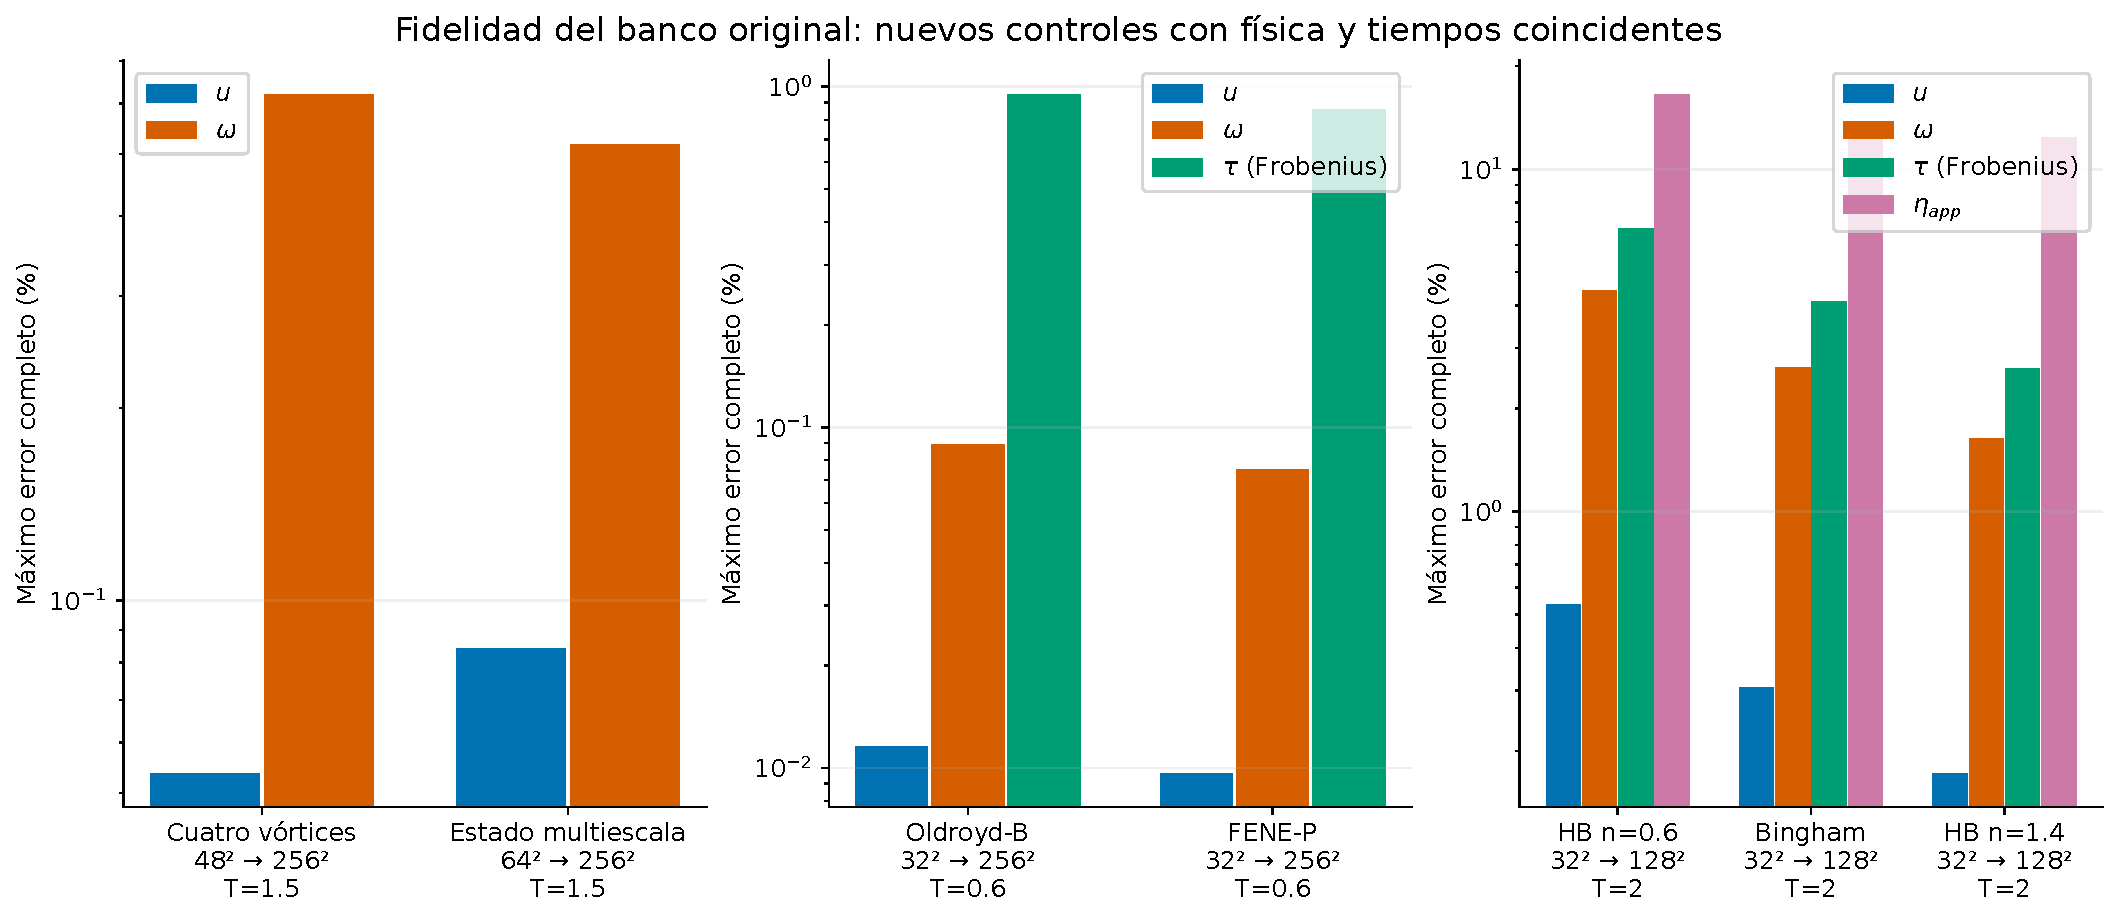
\includegraphics[width=\linewidth,height=.80\textwidth,keepaspectratio]{results/research/reference_fidelity_2026-10-14/figures/matching_original_references.pdf}
\caption{Calidad de las referencias históricas bajo su propia configuración física. Cambiar viscosidad, condición inicial o intervalo invalidaría atribuir el error al refinamiento de esa campaña. Los esfuerzos auxiliares juzgan la simulación aunque el estimador histórico sólo reconstruya velocidad.}
\label{fig:matched-original-references}\end{figure}
\end{landscape}
\clearpage

El reanálisis descriptivo conserva 2808 condiciones, 8424 mediciones de costo, 6 condiciones no convergentes y 23 uso de alternativa fbDMD$\to$TLS. En 66 de 216 observaciones no existe estimador admisible. Su rango cuatro, nueve ruidos y referencias de menor malla difieren del banco principal: no se combinan en una sola tasa ni se atribuye a la resolución el cambio entre configuraciones distintas.

En 1469 salidas históricas se cumple $e_u$$\leq$15~\% pero se incumple $e_\omega$$\leq$25~\%. Ese desacuerdo cuantifica por qué el error de velocidad aislado no basta para declarar fidelidad del flujo. Las salidas con divergencia impuesta tampoco certifican la ecuación de movimiento: un residuo de vorticidad medido entre instantáneas conserva error de muestreo y exige interpretación adicional.

\clearpage
\begin{landscape}
\begin{figure}[p]\centering
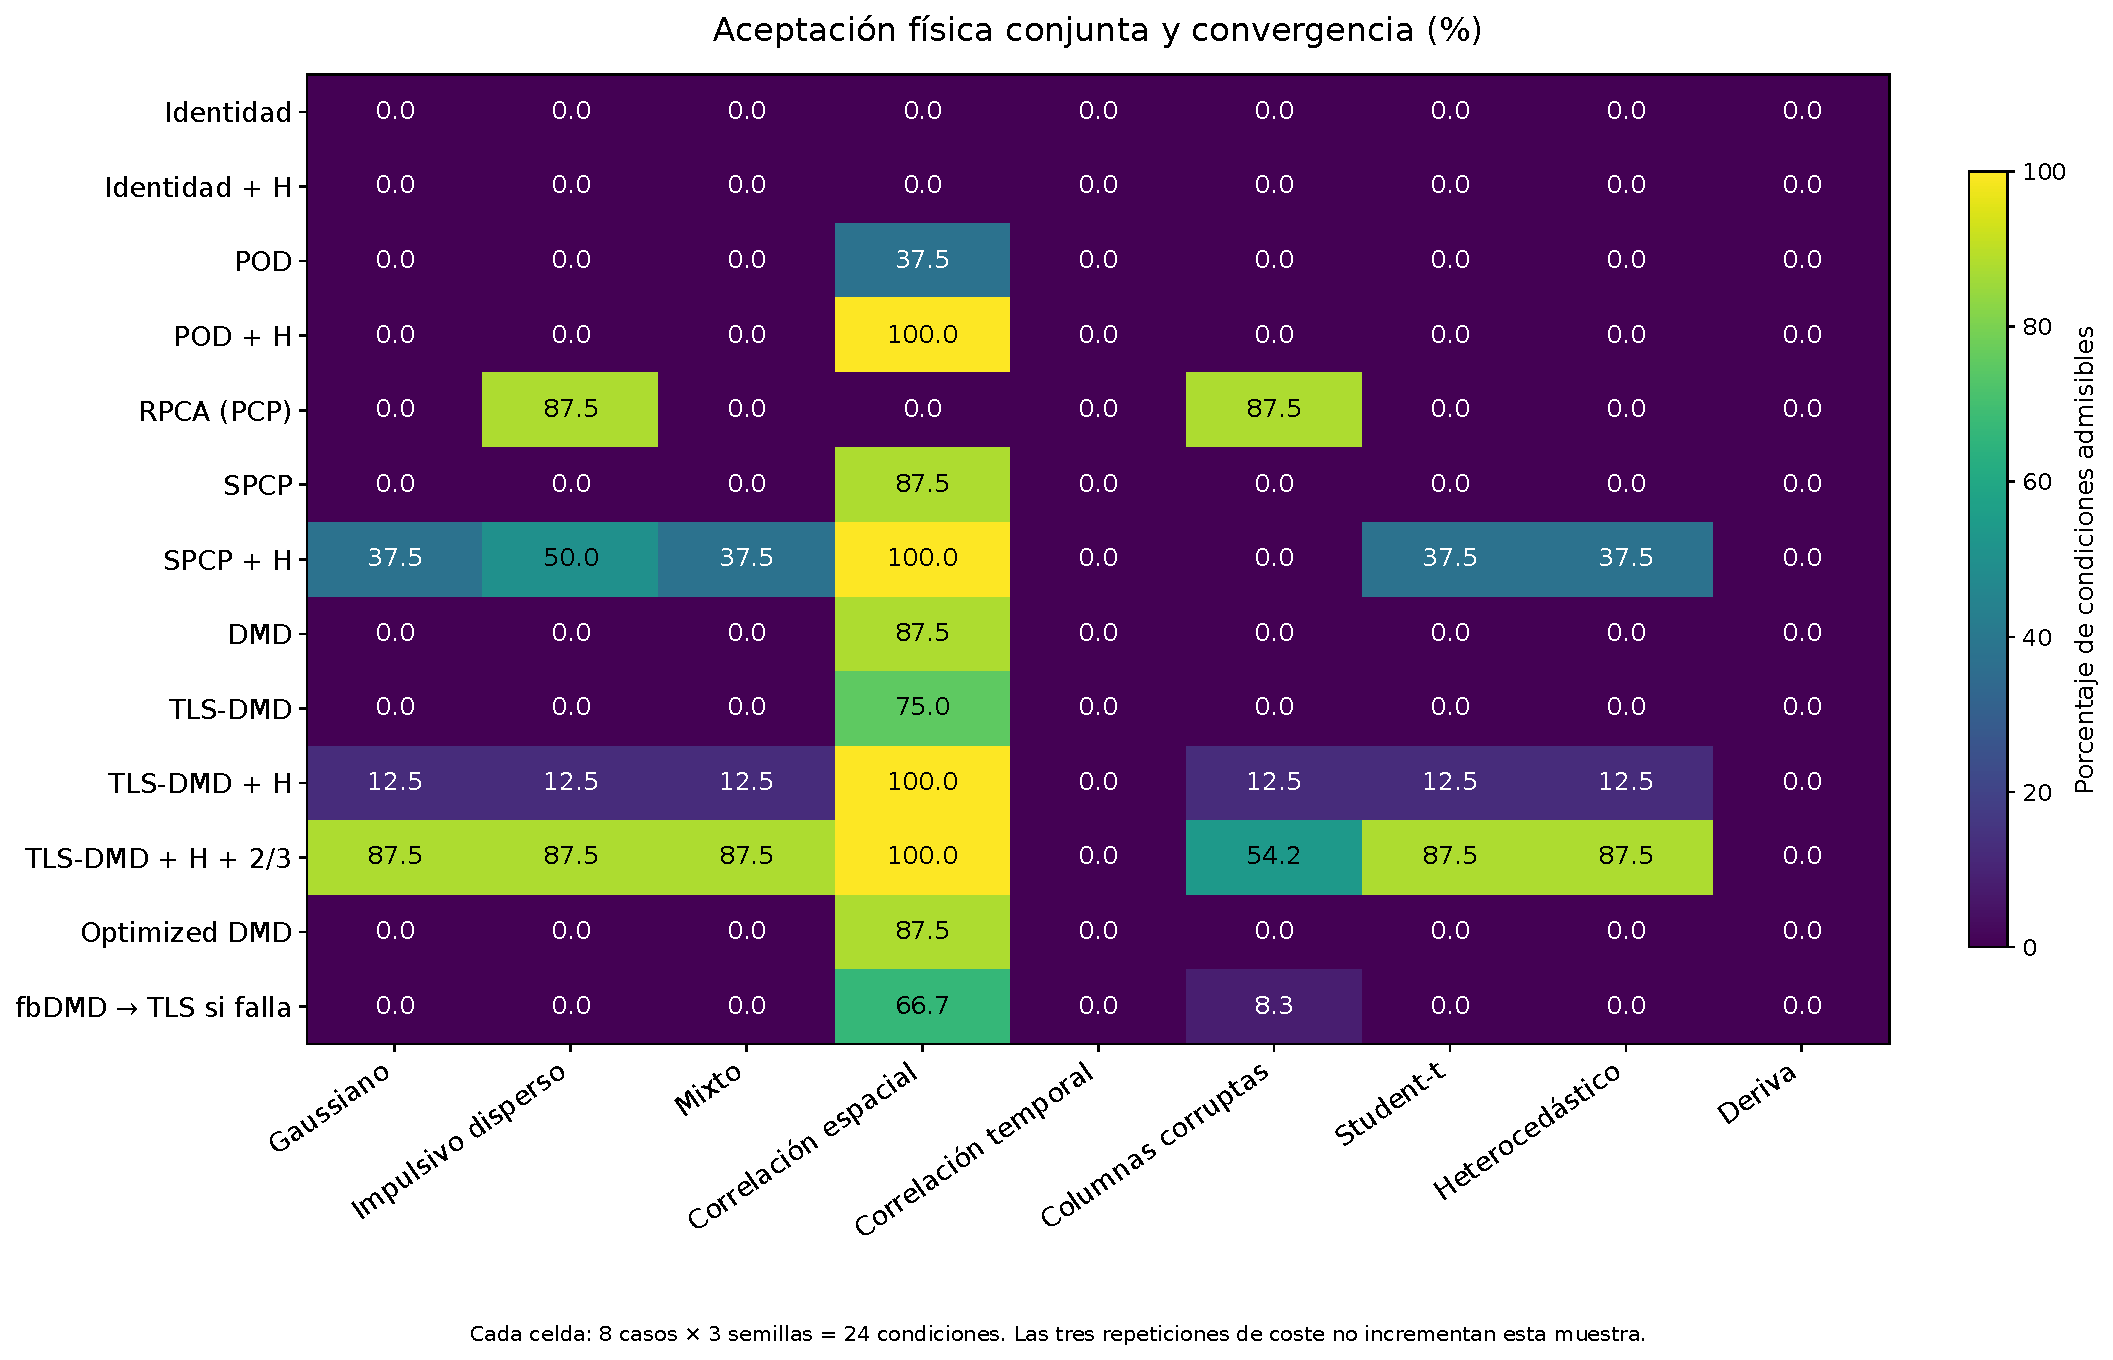
\includegraphics[width=\linewidth,height=.80\textwidth,keepaspectratio]{results/research/paired_model_comparison_2026-10-14/figures/acceptance_by_noise.pdf}
\caption{Cobertura del banco anterior en nueve contaminaciones. Cada celda cuenta 24 condiciones de calidad (ocho referencias y tres semillas); las tres mediciones de costo no aumentan ese número. Los parámetros y mallas difieren del banco principal, de modo que sus porcentajes se mantienen separados.}
\label{fig:historical-noise-coverage}\end{figure}
\end{landscape}
\clearpage

\begingroup\small\setlength{\tabcolsep}{3pt}
\begin{longtable}{@{}>{\raggedright\arraybackslash}p{5.5cm}>{\raggedright\arraybackslash}p{2.5cm}>{\raggedright\arraybackslash}p{2.0cm}>{\raggedright\arraybackslash}p{2.0cm}>{\raggedright\arraybackslash}p{2.4cm}@{}}
\caption{Ablaciones del banco amplio anterior con parámetros propios. La proyección H y el corte 2/3 no se equiparan al corte físico k\_c=10 del banco nuevo.}\\
\toprule
\textbf{Transición histórica} & \textbf{Admisibles} & \textbf{Rescata} & \textbf{Pierde} & \textbf{$\omega$ sin cambio} \\
\midrule\endfirsthead
\toprule
\textbf{Transición histórica} & \textbf{Admisibles} & \textbf{Rescata} & \textbf{Pierde} & \textbf{$\omega$ sin cambio} \\
\midrule\endhead
Identity $\to$ Identity + H & 0 $\to$ 0 & 0 & 0 & 216/216 \\
POD $\to$ POD + H & 9 $\to$ 24 & 15 & 0 & 216/216 \\
RPCA estable $\to$ RPCA estable + H & 21 $\to$ 72 & 51 & 0 & 216/216 \\
TLS-DMD $\to$ TLS-DMD + H & 18 $\to$ 42 & 24 & 0 & 216/216 \\
TLS-DMD + H $\to$ TLS-DMD + H + 2/3 & 42 $\to$ 142 & 100 & 0 & 24/216 \\
\bottomrule\end{longtable}\endgroup

\clearpage
\begin{landscape}
\begin{figure}[p]\centering
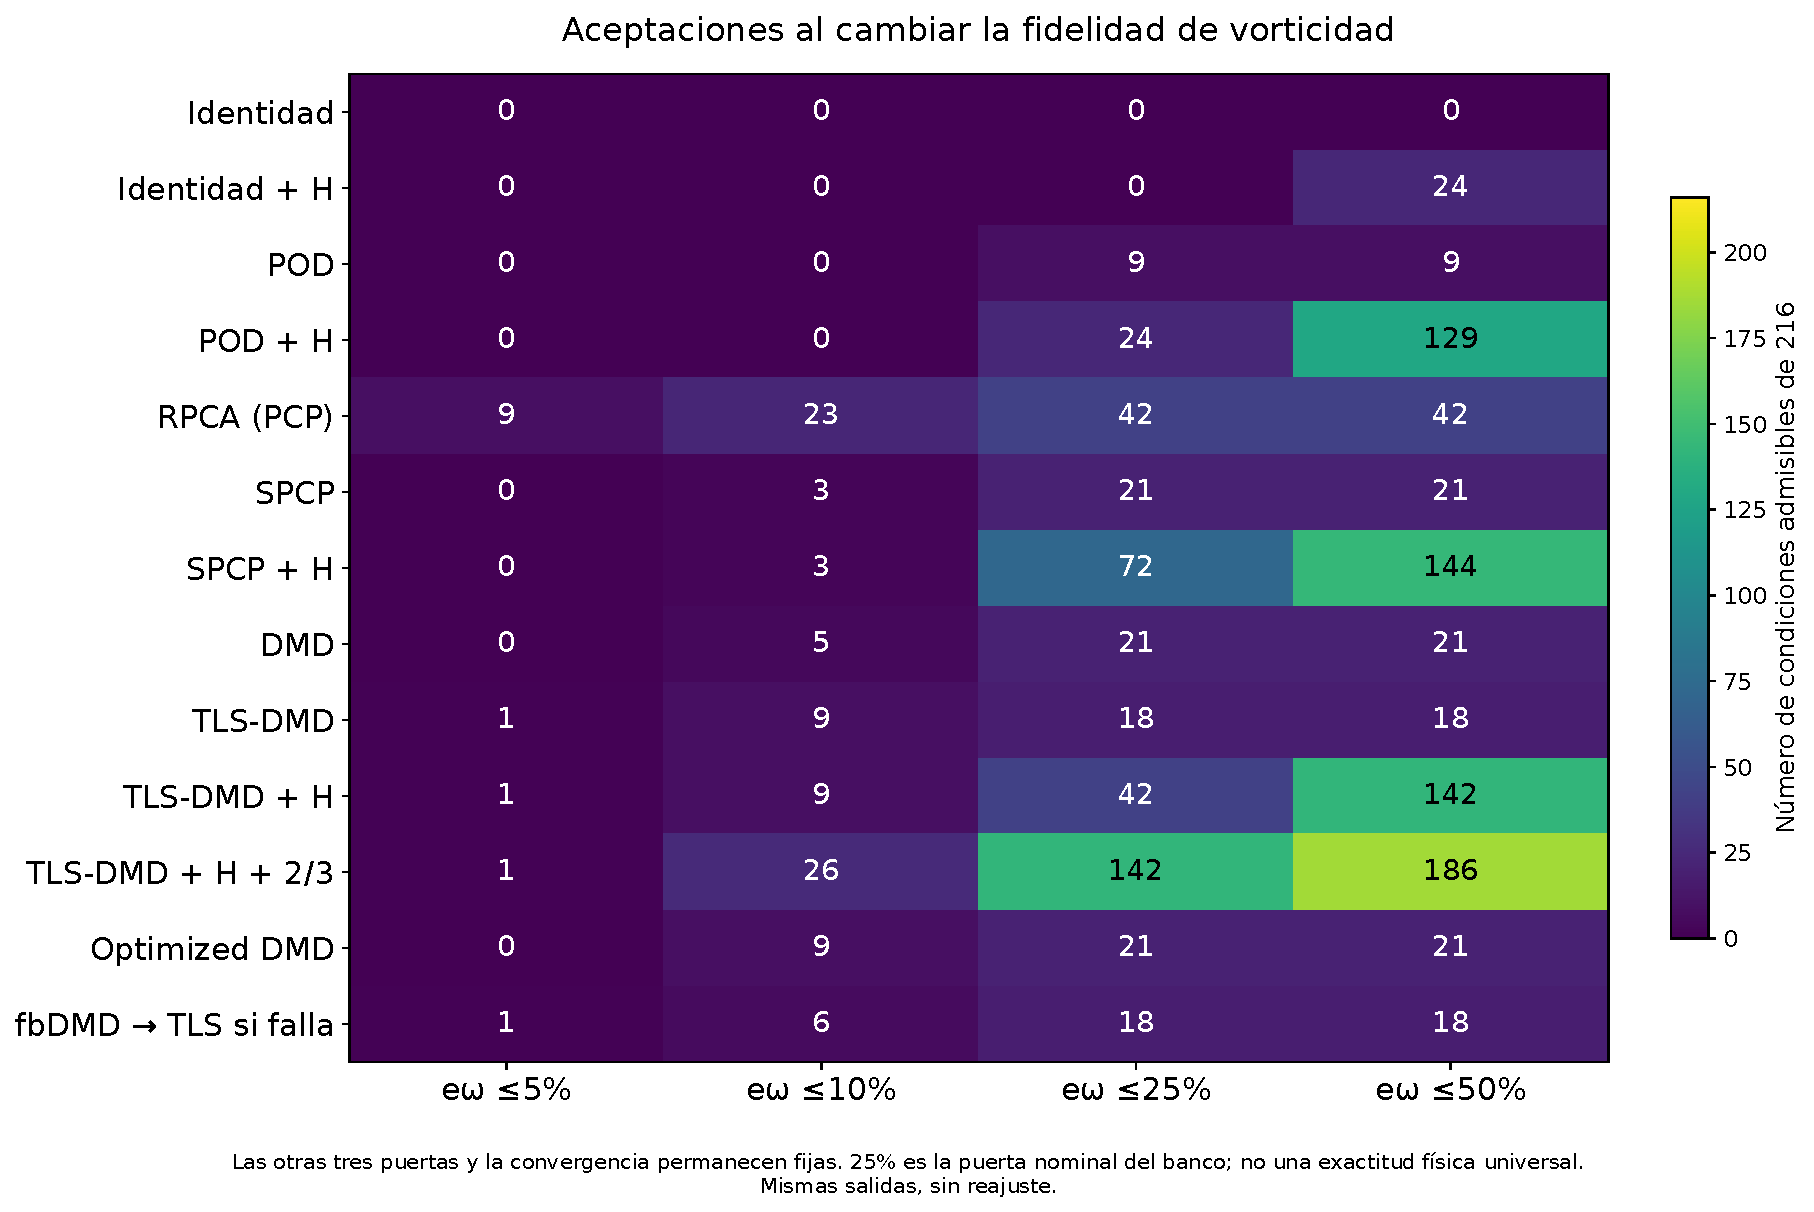
\includegraphics[width=\linewidth,height=.80\textwidth,keepaspectratio]{results/research/paired_model_comparison_2026-10-14/figures/tolerance_sensitivity_matrix.pdf}
\caption{Sensibilidad histórica a la tolerancia de vorticidad, manteniendo las demás puertas. Un conteo de aceptación depende del umbral declarado y debe acompañarse de errores continuos. Este análisis posterior no redefine las puertas con que se evaluó el banco principal.}
\label{fig:tolerance-sensitivity}\end{figure}
\end{landscape}
\clearpage

Las tres semillas exploran observaciones del mismo flujo; no estiman variabilidad entre condiciones iniciales, regímenes ni laboratorios. Las referencias son periódicas bidimensionales y la campaña reconstruye dentro de la ventana. No demuestra identificación de material, esfuerzo viscoelástico recuperado, pronóstico futuro, calle de vórtices externa ni generalización PIV. Los residuos de salida, los controles de resolución y los negativos anteriores permanecen separados y auditables.

\subsection{Acceso a la evidencia y lectura complementaria}

Las tablas de condición, resúmenes estratificados, ledger, hashes y figuras acompañan el capítulo. Los apéndices conservan el catálogo de evolución, el pronóstico cronológico y la tabla amplia histórica. La reproducción documental utiliza JSON/CSV y figuras publicadas; las trayectorias completas se regeneran con los scripts y se archivan por separado cuando exceden el límite por archivo de GitHub.
